%%%%%%%%%%%%%%%%%%%%%%%%%%%%%%%%%%%%%%%%%%%%%%%%%%%%%%%%%%%%%%%%%%%%%%%%%%%%%%%%
%%                           ONDER DE LOEP ARTIKEL                            %%
%%%%%%%%%%%%%%%%%%%%%%%%%%%%%%%%%%%%%%%%%%%%%%%%%%%%%%%%%%%%%%%%%%%%%%%%%%%%%%%%

\artikelfoto{Leerlijn GeoGebra}{}{Dennis Presotto\\Michel Roelens\\Mathias Stichelbaut\\Els Vanlommel}{img/geogebrascherm.png}


\startcontents[inhoudloep]	% om inhoud voor het loep artikel te beginnen

\begin{multicols}{2}
	
	\inhoudstafelloep			% om inhoudstafel voor het loep artikel te tonen
	
	%% Gebruik \section{titel} en \subsection{titel} om genummerde tussentitels te maken

 \section{Inleiding}

 In de loep van Uitwiskeling 38/3 hadden we het over de `grexit', de exit van de grafische rekenmachine. In steeds meer scholen hebben de leerlingen van de tweede en de derde graad geen grafische rekenmachine meer maar wel een laptop, een chromebook of een tablet. Vaak gebruiken de leerlingen daarnaast ook nog een klein, goedkoop rekenmachientje voor eenvoudige berekeningen.  Grafische computerprogramma's zoals GeoGebra, Desmos, Graphmatica... krijgen hierdoor een grotere rol toebedeeld. We kozen hier voor GeoGebra omdat het wijd verspreid is, gratis is en al lang zijn nut bewezen heeft. In deze loep overlopen we exemplarisch wat de leerlingen met GeoGebra in de wiskundeles kunnen doen in de verschillende graden van het secundair onderwijs.

 \subsection*{De rol van GeoGebra}

 Nu eens kunnen leerlingen met GeoGebra experimenteren om oplossingsideeën te krijgen. Dan weer kunnen ze er hun pen-en-papieroplossingen mee verifiëren. GeoGebra laat ook toe om soms een probleem grafisch op te lossen dat algebraïsch niet opgelost zou geraken. En bij bv. statistiek wordt het maken van berekeningen en diagrammen grotendeels aan de computer overgelaten om dan zelf te focussen op interpretatie en besluiten.

  Wij vinden GeoGebra en andere apps interessante hulpmiddelen omdat ze bijdragen tot het onderzoeken, begrijpen en visualiseren van de wiskundeleerstof. Werken met GeoGebra en andere software in de wiskundeles kan motiverend werken. Het is echter geen doel op zich. 

\subsection*{Wat staat er in deze loep?}
 We schetsen in grote lijnen een leerlijn en we voorzien in elke graad twee of drie lesactiviteiten. Het zijn lesactiviteiten waarin de leerlingen GeoGebra gebruiken, vertrekkend van het lege basisscherm. Voor de eerste graad vermelden we het gebruik van GeoGebra bij eigenschappen van vlakke figuren en zijn er lesactiviteiten over transformaties en over evenredige grootheden. Voor de tweede graad voorzien we een activiteit over bivariate statistiek en over ruimtemeetkunde. Voor de derde graad bespreken we algemene sinusfuncties, het berekenen van afgeleiden en integralen met o.a. het ComputerAlgebraSysteem van GeoGebra en het rekenen met matrices. In een appendix raken we heel kort enkele technische kwesties aan: GeoGebra op verschillende toestellen, GeoGebrabestanden online opslaan...

 \subsection*{Waar gaat deze loep niet over?}
 Je kunt GeoGebra ook gebruiken om mooie visualisaties te maken en voor de leerlingen te projecteren. Of je kunt als leraar kleine apps voor de leerlingen klaarmaken of online vinden. Dit is best interessant maar in deze loep hebben we het hier niet over.   Deze loep is ook geen handleiding over de technische kant van het werken met GeoGebra: waar staan welke knoppen in welke versie? Veel collega's hebben nog vragen over het gebruik van GeoGebra op toetsen en examens en over het toelaten van GeoGebra op smartphones. Ook binnen de redactie leven deze vragen; wij weten het ook niet altijd. Ook dit is niet het onderwerp van deze loep. 

 \subsection*{Een opmerking over de lesactiviteiten}
 Zoals vaak in Uitwiskeling, voorzien we lesactiviteiten met vragen en antwoorden. Een lesactiviteit kan een werktekst zijn om aan de leerlingen als opdracht te geven, maar meestal is het eerder een leidraad voor een stuk les gestuurd door de leerkracht. De vragen en antwoorden zijn een manier om concreet te maken hoe de les in interactie met de klas kan verlopen. De schuingedrukte antwoorden bevatten niet alleen mogelijke antwoorden van de leerlingen, maar soms ook bijkomende informatie voor de leerkracht in verband met de gestelde vraag.

\end{multicols}
\afbeelding[10cm]{tekeningenKurt/UWgeogebra.jpg}{}{fig:geoegebra} 
\begin{multicols}{2}
 
 \section{Eerste graad}

\subsection{Eigenschappen van vlakke figuren onderzoeken}

In de eerste graad worden speciale driehoeken en vierhoeken bestudeerd: de definities, de omtrek, de oppervlakte, speciale lijnen hierin, eigenschappen over de diagonalen... 

Om eigenschappen te ontdekken, is een nauwkeurige GeoGebrafiguur betrouwbaarder dan een schets op papier. Bovendien kun je de gemaakte figuur nog wijzigen. De figuren die je maakt, zijn dynamisch.

Stel dat leerlingen eigenschappen van de diagonalen willen ontdekken in een parallellogram, een rechthoek en een ruit. 

Eerst moeten ze deze figuren in GeoGebra tekenen. Daarvoor moeten ze heel bewust steunen op de definities, want er zijn geen knoppen voorzien voor parallellogrammen, rechthoeken en ruiten. Bv. om een parallellogram te maken, moeten ze twee aansluitende zijden tekenen en dan de knop \emph{Evenwijdige rechte} gebruiken om de twee andere zijden te maken (\autoref{Geo Parallellogram}). Het snijpunt hiervan is het vierde hoekpunt van het parallellogram.

Wat je in GeoGebra niet mag doen, is de punten op het zicht plaatsen (`mikken'). Zelfs al zou je erin slagen om heel goed te mikken, de figuur zal zijn eigenschappen verliezen wanneer je de vrije punten verplaatst. Het is goed dat leerlingen dit aspect van GeoGebra van in de eerste graad leren.

\afbeelding[4cm]{img/geo1.JPG}{Een parallellogram is een vierhoek met twee paar evenwijdige zijden.}{Geo Parallellogram}

Nadat de leerlingen met lijnstukken of met de knop \emph{Veelhoek} het parallellogram getekend hebben, verbergen ze best de uitstekende `sprieten' van de evenwijdige rechten door \emph{Object tonen} af te vinken voor deze rechten.

Analoog gebruiken ze voor een rechthoek de knop \emph{Loodlijn}. Voor een ruit kunnen ze met cirkels werken of met de knop \emph{Passer} (\autoref{Geo ruit}). 


\afbeelding[3.7cm]{img/geo2bis}{Een ruit is een vierhoek met vier even lange zijden}{Geo ruit}{}


Eens de vierhoek getekend is en de constructielijnen verborgen zijn, kunnen de leerlingen aan het onderzoek van de diagonalen starten. Ze proberen een eigenschap vast te stellen en te formuleren. Het is belangrijk te benadrukken dat een eigenschap enkel geldt als ze waar is voor alle voorbeelden van de figuur. In GeoGebra kan men dit controleren door aan de `vrije' hoekpunten te trekken en zo de figuur te veranderen.

\subsection{Vlakke transformaties}

In het tweede jaar maken de leerlingen binnen meetkunde kennis met enkele transformaties van het vlak (en van de ruimte): verschuivingen, draaiingen, spiegelingen... Best toon je de leerlingen ook eens een transformatie die de figuren vervormt, want het begrip meetkundige transformatie is veel ruimer dan enkel de isometrieën.

Hier beperken we ons tot draaiingen van het vlak. GeoGebra is hiervoor bijzonder geschikt. Je kunt dit analoog uitwerken voor andere transformaties. In de lesactiviteit hieronder maken we duidelijk dat wat wiskundigen onder een draaiing verstaan niet hetzelfde is als wanneer je iets draait buiten de wiskunde.
 
 Deze activiteit gaat vooraf aan het zelf tekenen van het draaibeeld van een figuur. We starten met het draaien van een volledige figuur en dan focussen we op wat er gebeurd is met de individuele punten. Dit kunnen leerlingen dan gebruiken om ook zelf op papier het draaibeeld van een figuur te bepalen. De nieuwe minimumdoelen leggen minder nadruk op dat zelf tekenen dan op het begrijpen hoe draaiingen (en andere transformaties) in elkaar zitten. Het is niet de bedoeling om het zelf tekenen echt te `trainen', maar het speelt wel een rol in het begrijpen wat een draaiing is.

\end{multicols}

\begin{lesactiviteit}{Een draaiing op papier en in GeoGebra}

\begin{vraagenantwoord}

  \vraag{Teken met de losse hand een dier op een blaadje papier zonder je pen op te heffen en knip het uit. Kies een punt binnen die figuur, plaats daar de naald van je passer en draai de figuur rond dat punt over een hoek van (ongeveer) 50° in tegenwijzerzin.}

  \antwoord{De leerlingen doen dat.}

  \afbeelding[4cm]{img/visgedraaid.JPG}{}{}{}

  \vraag{Nu willen we hetzelfde doen in GeoGebra. Draaien heet in GeoGebra `roteren'; een rotatie is een draaiing. Je tekent het dier in GeoGebra, met de knop \emph{Pen}, zonder je `pen' op te heffen. De tekening hoeft niet perfect te zijn. Je duidt  een punt $C$ aan binnen de figuur; dat is het `draaicentrum', de tegenhanger van de passernaald. Draai de figuur met de knop \emph{Roteer rond punt}. Je klikt op de figuur en op het punt $C$ en je vult de draaihoek in, 50° in tegenwijzerzin. Geef de oorspronkelijke figuur en het `draaibeeld' verschillende kleuren.}

  \antwoord{Hieronder zie je in het groen de originele figuur. Ter informatie: het stelt een vis voor. Het draaibeeld hebben we paars gekleurd. Merk op: als je tekent zonder je pen op te heffen, ben je zeker dat GeoGebra je tekening als één geheel draait. Als je je pen opheft, is het mogelijk (maar niet zeker) dat GeoGebra je tekening als twee of meer aparte figuren opvat.}

  \afbeelding[4cm]{img/geo2.JPG}{}{}

  \vraag{Vergelijk wat je op het scherm zag gebeuren met wat je zag als je de papieren figuur rond de passernaald draaide. Wat is er anders?}

  \antwoord{In GeoGebra blijft de originele figuur staan en is het draaibeeld een nieuwe figuur. Bij de figuur in papier is de oorspronkelijke figuur zelf gedraaid en is die er niet meer op de oorspronkelijke plaats. Nog een verschil is dat in GeoGebra het beeld onmiddellijk verschijnt terwijl de papieren figuur een baan aflegt.}

  \vraag{Verplaats in de GeoGebrafiguur het centrum $C$ buiten de tekening van het dier. Kun je hiermee nog een ander verschil benoemen tussen het draaien in GeoGebra en in de realiteit?}

  \antwoord{In GeoGebra kun je de figuur even goed rond een punt binnen als buiten de getekende figuur draaien. Bij de papieren figuur moet je de naald van de passer binnen de uitgeknipte figuur prikken om er rond te draaien. Wat wel kan, is de figuur niet uitknippen en de naald buiten de figuur maar wel op het blad prikken. Dan draai je het hele blad en de figuur gaat mee. Iets dergelijks gebeurt in GeoGebra, alsof het hele vlak een reusachtig blad papier is dat ronddraait.}
 
   \afbeelding[4,5cm]{img/geo3.JPG}{}{}
  
\end{vraagenantwoord}

\begin{kader}{}{}
    Als je in de wiskunde en in GeoGebra een figuur draait rond een punt (het `draaicentrum') over een bepaalde `draaihoek', dan blijft de figuur staan en ontstaat er een nieuwe figuur, het `draaibeeld' van de figuur. Eigenlijk wordt niet enkel de figuur gedraaid, maar alle punten van het vlak, ook buiten de tekening.
\end{kader}

Om zelf het draaibeeld van een meetkundige figuur, bv. een driehoek te kunnen tekenen, is het nuttig om te weten waar het draaibeeld van elk willekeurig punt van het vlak terechtkomt. Dan kunnen we dat toepassen op de hoekpunten van de driehoek.

\begin{vraagenantwoord}[resume]
\vraag{Teken een punt $P$ en laat GeoGebra dat punt draaien net zoals dat met de figuur gebeurde (zelfde centrum $C$, zelfde `draaihoek' 50° in tegenwijzerzin). Het draaibeeld van $P$ is $P'$. Verbind zowel $P$ als $P'$ met $C$ door lijnstukken. Leg nauwkeurig uit waar $P'$ ligt ten opzichte van $C$ en $P$. Aanwijzing: welke afstanden zijn gelijk? Welke hoek is gelijk aan de draaihoek 50°?}

\antwoord{Het punt $P'$ ligt even ver van $C$ als het punt $P$. Anders gezegd: $|CP|=|CP'|$. Bovendien is de hoek $\angle PCP'$ gelijk aan 50° in tegenwijzerzin.}

   \afbeelding[5cm]{img/geo4.JPG}{}{}

\end{vraagenantwoord}

\begin{kader}{}{}
Bij een draaiing rond een centrum $C$ over een georiënteerde hoek $\alpha$ krijgt elk punt $P$ van het vlak een beeld $P'$ zo dat $|CP'|=|CP|$ en $\angle PCP'=\alpha$. Voor het punt $C$ zelf moeten we hierbij een uitzondering maken, het wordt op zichzelf afgebeeld.
\end{kader}

\begin{vraagenantwoord}[resume]

    \vraag{Teken op een blad papier een willekeurige vierhoek en een willekeurig draaicentrum. Draai de vierhoek over 25° in wijzerzin.}

    \antwoord{De leerlingen tekenen de draaibeelden van de vier hoekpunten. Om ervoor te zorgen dat de afstanden tot het centrum gelijk zijn, kunnen ze meten of de passer gebruiken. Voor de hoek gebruiken ze de gradenboog van de geodriehoek. Dan verbinden ze de draaibeelden van de hoekpunten om het draaibeeld van de vierhoek te tekenen.}

    \emph{Mogen ze gewoon die vier punten zomaar verbinden door lijnstukken? Dit bespreken we hieronder buiten de lesactiviteit.}
\end{vraagenantwoord}
    
\end{lesactiviteit}

\begin{multicols}{2}

\subsection*{Opmerking voor de leerkracht}
 Je zou kunnen ingaan op de eigenschap: `het draaibeeld van een lijnstuk is een lijnstuk'. Maar is dit zinvol voor de leerlingen van de eerste graad?\\ 
 De bepaling van het beeld van een willekeurig punt $P$ van het vlak is het `voorschrift' van de transformatie, net zoals je bij een reële functie het beeld van een willekeurig getal $x$ bepaalt. Het beeld van een figuur (rechte, driehoek, vis...) is dan de verzameling (meetkundige plaats) van de beelden van alle punten van de figuur. In een theoretische aanpak is dit de definitie van een draaiing en is het draaien van de tekening van het dier enkel een inleiding. In deze theoretische aanpak moet je bewijzen dat het draaibeeld van een lijnstuk opnieuw een lijnstuk is. 

De leerlingen van de eerste graad bekijken het niet zo theoretisch. Voor hen is het vastleggen van het beeld van een willekeurig punt geen definitie maar een opstap naar het zelf tekenen van draaibeelden. Een draaiing blijft voor hen verbonden met het concrete draaien in de werkelijkheid, ook al zijn een aantal verschilpunten met hen besproken. En bij het draaien in de werkelijkheid is het evident dat het draaibeeld van een lijnstuk een lijnstuk is en niet vervormd is. We denken dat het in de eerste graad te vroeg is om de theoretische aanpak aan te kaarten.

\subsection{Evenredige grootheden}

In Uitwiskeling 27/4 vind je een loep over evenredigheden. We beperken ons hier tot een korte situering met de focus op het gebruik van GeoGebra. Vooraf: met `evenredig' bedoelen we `recht-evenredig' en niet `omgekeerd-evenredig'.

Verhoudingstabellen kwamen al aan bod in de lagere school en in het eerste jaar en worden in het tweede jaar herhaald, bijvoorbeeld als volgt. 

Als je pannenkoeken bakt voor 3 personen heb je 250 g bloem nodig (en ook 2 eieren en 0,5 l melk). Dan heb je voor 6 personen 500 g bloem nodig en voor 15 personen 1250 g bloem. Je kunt een verhoudingstabel maken met een rij voor het aantal personen en een rij voor de hoeveelheid bloem (en rijen voor de eieren en de melk maar die laten wij hier weg). Als je het aantal personen met een getal vermenigvuldigt, wordt de hoeveelheid bloem met hetzelfde getal vermenigvuldigd. We zeggen dat de hoeveelheid bloem evenredig (of: recht-evenredig) is met het aantal eters. Een gevolg hiervan is dat de hoeveelheid bloem per persoon, de verhouding van getallen boven elkaar in de tabel, constant is: $\displaystyle\frac{250}{3}=\frac{500}{6}=\frac{1250}{15}$.


\begin{tabel}
		\begin{tabular}{m{4cm} C{.6cm} C{.8cm} C{1cm} C{1.1cm}}  % tekstbreedte=7.5cm, elke tabelkolom = breedte + 2x1mm marge (2x want marge links & rechts)
			\hlinethick  % dikkere lijn, gebruik deze rond de hoofding (eerste rij) en om de tabel te eindigen
			
			Aantal personen  & 3 & 6 & 15 \\
			
			\hline
			Hoeveelheid bloem (in g)
			\quad & 250 & 500 & 1250  \\
			
			\hlinethick
		\end{tabular}
		\caption{Verhoudingstabel bloem voor pannenkoeken}\label{tab:vbmulticol}
	\end{tabel}


In het tweede jaar komen daar grafieken en formules bij. Hier kan GeoGebra nuttig zijn.

\end{multicols}

\begin{lesactiviteit}{Evenredige grootheden grafisch onderzoeken}

Men zegt dat twee rechthoeken dezelfde vorm hebben als ze dezelfde verhouding $\frac{\text{lengte}}{\text{breedte}}$ hebben. Zo heeft een rechthoek van $6$ bij $4$ dezelfde vorm als een rechthoek van $4,5$ bij $3$ want
$$\frac{6}{4}=\frac{4,5}{3}.$$

\begin{vraagenantwoord}
\vraag{Teken op papier een rechthoek van 6 cm bij 4 cm en een rechthoek van 4,5 cm bij 3 cm. Knip ze uit. Leg ze op elkaar, de kleinste op de grootste, met één hoekpunt samenvallend en de zijden aan dat hoekpunt op elkaar. Wat valt er op? Controleer eventueel met nog een derde rechthoek.}

\antwoord{De diagonalen liggen op elkaar. Of nog: de overstaande hoekpunten van het samenvallende hoekpunt liggen op één rechte met dat samenvallende hoekpunt.}

\afbeelding[4cm]{img/rechthoeken.JPG}{}{}{}

\vraag{Als je het samenvallende hoekpunt in de oorsprong van een assenstelsel plaatst en de zijden aan dat hoekpunt op de assen, wat zijn dan de coördinaten van de hoekpunten van de rechthoeken?}
\antwoord{Als je de langste zijden op de $x$-as plaatst en als eenheid op de assen ook de centimeter neemt, dan hebben de hoekpunten van de grootste rechthoek coördinaten $(0, 0), (6, 0), (6, 4), (0, 4)$ en die van de kleinste rechthoek $(0, 0), (4,5; 0), (4,5; 3), (0, 3)$.}

\vraag{Hoe kun je door de punten met deze coördinaten in een assenstelsel te tekenen, vaststellen dat de lengtes en de breedtes van deze rechthoeken evenredig zijn?}

\antwoord{Door na te gaan dat de punten $(0, 0), (4,5; 3)$ en $(6, 4)$ op één rechte liggen.}

\end{vraagenantwoord}

\begin{kader}{}{}
Rechthoeken hebben dezelfde vorm als hun breedte en lengte (recht-)evenredig zijn. Je kunt zien of dit het geval is door voor elke rechthoek het punt $(\text{lengte}, \;\text{breedte})$ in een assenstelsel te tekenen. De lengte en de breedte zijn evenredig als deze punten op een rechte door de oorsprong gelegen zijn.
\end{kader}


Hieronder zie je de afmetingen van enkele smartphones Samsung Galaxy. We gaan na of ze dezelfde vorm hebben.

\begin{tabel}
		\begin{tabular}{m{2cm} C{2cm} C{2cm} C{2cm} C{2cm}}  % 
			\hlinethick  
			\tableheader{} & \tableheader{S22} & \tableheader{S22 Plus} & \tableheader{S22 Ultra}  \\ 
			\hlinethick

			Breedte & 7,06 cm & 7,58 cm & 7,79 cm  \\
   			Hoogte  & 14,6 cm & 15,74 cm & 16,33 cm  \\
			Massa  & 167 g & 195 g & 228 g \\
			\hlinethick
		\end{tabular}
		
	\end{tabel}

\begin{vraagenantwoord}[resume]

\vraag{Teken in GeoGebra een grafiek om te controleren of de breedte en de hoogte van deze toestellen evenredig zijn.}

\antwoord{De grafiek hieronder toont de respectievelijke punten met coördinaten \emph{(breedte, hoogte)} van de drie modellen. Dat mocht natuurlijk ook \emph{(hoogte, breedte)} zijn, zolang dezelfde keuze wordt gemaakt voor alle drie. In het groen is de rechte getekend die de oorsprong verbindt met het punt S22. De punten lijken op de groene rechte te liggen en dus lijken de breedte en de hoogte van deze drie toestellen evenredig te zijn. Maar als we inzoomen (tweede grafiek hieronder) zien we dat  dit maar bij benadering geldt.}

\afbeelding[4.5cm]{img/geo5.png}{}{}

\afbeelding[5.4cm]{img/geo5inzoom.png}{}{}

\vraag{Is de breedte bij deze drie smartphones evenredig met de massa?}

\antwoord{Hieronder zie je de grafiek met horizontaal de breedte en verticaal de massa van deze toestellen. De groene rechte is weer de rechte die de oorsprong verbindt met het punt van S22. Nu is er overduidelijk geen evenredigheid tussen de massa en de breedte. De grotere toestellen zijn in verhouding duidelijk zwaarder.} 

\emph{Aan oudere leerlingen zou je kunnen vragen of dit te voorspellen was. Als de toestellen ongeveer gelijkvormige balken zijn en als de massadichtheid ongeveer dezelfde is, dan zou de massa ongeveer evenredig moeten zijn met de derde macht van de breedte. We zouden in plaats van een rechte de grafiek van een derdegraadsfunctie door de oorsprong en de drie punten moeten tekenen. Maar deze opmerking komt voor leerlingen van de eerste graad te vroeg...}

\afbeelding[7cm]{img/geo6.png}{}{}
    
\end{vraagenantwoord}

In het vorige zagen we dat de punten met als coördinaat (lengte, breedte) bij gelijkvormige rechthoeken op een zelfde rechte liggen door de oorsprong. Lengte en breedte zijn bij dergelijke rechthoeken evenredige grootheden. In de volgende vragen verlaten we het verhaal van de rechthoeken. We zullen vaststellen dat ook bij andere evenredige grootheden de punten op één rechte door de oorsprong gelegen zijn.

Met 5 liter verf kun je $72\;\text{m}^2$ muur verven. De hoeveelheid verf die je nodig hebt, is evenredig met de muuroppervlakte. 

\begin{vraagenantwoord}[resume]
     \vraag{Vul de tabel aan en teken de punten in een assenstelsel in GeoGebra.}

     \begin{tabel}
		\begin{tabular}{m{4cm} C{1cm} C{1cm} C{1cm} C{1cm}C{1cm}}  
			\hlinethick

			Muuroppervlakte (in $\text{m}^2$) & 36 & 72 & 144&  \\
   \hline
   			Hoeveelheid verf (in l)  & & 5 & &25  \\
		
			\hlinethick
		\end{tabular}
	\end{tabel}
\vspace{1cm}
 \antwoord{Hieronder vind je de ingevulde tabel en de grafiek. Om de punten mooi in beeld te krijgen, moeten de leerlingen apart uitzoomen in de $x$- en de $y$-richting. Dit gebeurt door aan de $x$-as en de $y$-as te `trekken' met de knop \emph{Tekenvenster verplaatsen}. De leerlingen stellen vast dat de punten op een rechte door de oorsprong liggen. Hier dient de grafiek niet om na te gaan of beide grootheden evenredig zijn, want daar zijn ze van uit gegaan bij het invullen van de tabel.}

\begin{tabel}
		\begin{tabular}{m{4cm} C{1cm} C{1cm} C{1cm} C{1cm}C{1cm}}  
			\hlinethick

			Muuroppervlakte (in $\text{m}^2$) & 36 & 72 & 144&  \textbf{360}\\
            \hline
   			Hoeveelheid verf (in l)  & \textbf{2,5}& 5 & \textbf{10}&25  \\
		
			\hlinethick
		\end{tabular}
	\end{tabel}

     \afbeelding[9cm]{img/grafiek verf.png}{}{}{}

     \vraag{Hoeveel verf heb je nodig voor $x\;\text{m}^2$ muur?}
     \antwoord{De factor waarmee de getallen van de eerste rij van de tabel vermenigvuldigd worden om naar de tweede rij te gaan, is constant en is gelijk aan $\frac{5}{72}$. Dit geldt niet alleen voor de $x$-waarden die in de tabel staan. Dus: voor $x\; \emph{m}^2$ muur heb je $\frac{5}{72}\cdot x \;\text{liter}$ verf nodig.}

     \vraag{Wat is het verband tussen $x$ en $y$ als $(x, y)$ een punt is van de getekende rechte?}

     \antwoord{Het verband is: $y=\frac{5}{72}x$. Eventueel kunnen leerlingen dit controleren door een willekeurig (lopend) punt op de rechte te nemen. Ook kunnen ze vaststellen dat punten buiten de rechte hier niet aan voldoen.}

     \vraag{Hoeveel verf heb je nodig om een muur van  $1000\;\text{m}^2$ te verven?}

     \antwoord{Invullen geeft: $\frac{5}{72}\cdot 1000= \frac{625}{9}\approx 69,44$ liter verf.}

     \vraag{Open in GeoGebra een nieuw grafiekblad. Geef de formule $y=k x$ in. GeoGebra zal een schuifbalk maken voor de waarde van $k$. Wat gebeurt er als $k$ verandert? Je mag je beperken tot $k>0$.}

     \antwoord{De leerlingen stellen vast dat de grafiek voor elke waarde van $k$ een rechte door de oorsprong is. Als $k$ positief is, stijgt de rechte (en als $k$ negatief is, daalt die, maar dat is hier niet de bedoeling). Door het domein van de schuifbalk aan te passen, kunnen ze ervoor zorgen dat $k$ enkel positief kan zijn. Leerlingen stellen vast: hoe groter $k$ hoe 'steiler' de grafiek. }

     \afbeelding[9cm]{img/kx.png}{}{}{}

     \emph{Afhankelijk van de GeoGebra-versie komt de schuifbalk in het algebravenster of op de tekening.}

     \vraag{Bij welke waarde van $x$ kun je de waarde van $k$ aflezen op de grafiek als de $y$-waarde? Teken op die plaats een verticaal lijnstuk van lengte $k$.}

     \antwoord{Voor $x=1$ krijg je door in te vullen in de formule $y=k\cdot 1=k$. Dus: bij $x=1$. Het punt van de grafiek bij $x=1$ is het punt $(1, k)$. De leerlingen tekenen op de grafiek het lijnstuk dat $(1, 0)$ verbindt met $(1, k)$.}
     
\end{vraagenantwoord}

\begin{kader}{}{}
Je kunt een evenredig verband tussen twee grootheden $x$ en $y$ voorstellen door een formule van de vorm $y=k\cdot x$ waarbij $k$ de vaste factor is om in de tabel van een waarde van $x$ naar de overeenkomstige waarde van $y$ te gaan. Men noemt de formule ook de `vergelijking' van de rechte door de oorsprong. Op de grafiek is $k$ de hoogte van het punt van de grafiek recht boven $1$ op de $x$-as. Hoe groter $k$, hoe steiler de grafiek.
\end{kader}

\end{lesactiviteit}

\begin{multicols}{2}

Bij de laatste vraag kwam even een schuifknop aan bod, om de parameter $k$ te kunnen variëren. Om vanuit een gegeven tabel van evenredige grootheden de grafiek te tekenen, heb je geen schuifknop nodig. Je kunt immers twee punten verbinden (bv. de oorsprong en één van de punten uit de tabel). Dit is anders bij omgekeerd-evenredige grootheden...

\subsection*{Omgekeerd-evenredigheid}

Bij een `omgekeerd-evenredig' verband is de grafiek een hyperbool. In de tabel is niet de verhouding maar wel het product van overeenkomstige waarden  constant. Vaak is dat vaste product bij voorbaat gekend. Neem het voorbeeld van de `dodentocht', de wandeling van 100 km rond de gemeente Bornem. Dan zijn de wandeltijd $t$ van iemand die de hele wandeling maakt en de gemiddelde wandelsnelheid  $v$ van deze wandelaar omgekeerd-evenredig, want het product is 100 km. De formule is $v=\frac{100\;\text{km}}{t}$.  In het voorbeeld van rechthoeken met een zelfde oppervlakte zijn de lengte en de breedte omgekeerd-evenredig want het product is die vaste oppervlakte.


Als je een tabel krijgt zoals \autoref{tab:Omgekeerd}, dan zie je meteen dat het verband dalend is: hoe groter $x$, hoe kleiner $y$. Het verband is alvast geen \mbox{(recht-)}evenredigheid. Maar, net zoals niet elk stijgend verband een (recht-)evenredigheid is, is een dalend verband niet noodzakelijk een omgekeerd-evenredigheid! 

\begin{tabel}
		\begin{tabular}{m{0.8cm} C{0.8cm} C{0.8cm} C{0.8cm} C{0.8cm}C{0.8cm}C{0.8cm}  }  
			\hlinethick

			$x$ & 0,40 & 0,50 & 2,50&1,40&3,30&4,00  \\
            \hline
   			$y$ & 3,50&2,80&0,56&1,00&0,50&0,48\\
		
			\hlinethick
		\end{tabular}
  \caption{Zijn de grootheden $x$ en $y$ omgekeerd-evenredig?}
  \label{tab:Omgekeerd}
  
	\end{tabel}

Om uit te zoeken of $x$ en $y$ omgekeerd-evenredig zijn, kun je  alle producten van overeenkomstige waarden vergelijken. Of: je kunt het grafisch doen. Teken de punten in een assenstelsel, maak een grafiek met de formule $y=\frac{k}{x}$, waarbij GeoGebra voor $k$ een schuifbalk maakt en kijk of je $k$ zo kunt schuiven dat de grafiek door de punten gaat.  

\afbeelding[5cm]{img/omgekeerd1.JPG}{Omgekeerd-evenredigheid grafisch nagaan}{Geo omgekeerd1}
\afbeelding[5cm]{img/omgekeerd2.JPG}{Omgekeerd-evenredigheid grafisch nagaan}{Geo omgekeerd2}

Op \autoref{Geo omgekeerd1} zie je dat de eerste punten mooi op de hyperbool $y=\frac{1,4}{x}$ liggen, maar de laatste twee punten ontsnappen hieraan... Door verder te schuiven met $k$ kun je de laatste twee punten  wel ongeveer op de grafiek krijgen, maar dan liggen de eerste vier punten er niet meer op (\autoref{Geo omgekeerd2}).

In de volgende paragrafen voor de tweede graad, worden GeoGebraknoppen gebruikt om automatisch een regressierechte of -kromme te tekenen als model voor een puntenwolk. Dit gebruiken we hier in de eerste graad bewust niet.
    

 \section{Tweede graad}



In de tweede graad kan GeoGebra op verschillende plaatsen zinvol ingezet worden. Zo kunnen leerlingen op analoge manier als hierboven bij de evenredigheden het effect van parameters bij eerste- en tweedegraadsfuncties met schuifknoppen onderzoeken. Dat behandelen we niet in deze loep. In de paragraaf over de derde graad komen we wel terug op het werken met schuifknoppen bij het onderdeel over de algemene sinusfunctie.

Ook in vlakke meetkunde is het voor de hand liggend dat GeoGebra opnieuw door leerlingen kan worden gebruikt om snel nauwkeurige dynamische tekeningen te maken als hulpmiddel bij het oplossen van problemen of bij het onderzoeken van eigenschappen. We denken hier bijvoorbeeld aan het onderdeel van de cirkel, met o.a. eigenschappen van middelpunts- en omtrekshoeken. Ook in het kader van de stelling van Pythagoras kun je Geo\-Gebra inzetten. In Uitwiskeling 15/2 (1999) stelden we de vraag bij welke driehoeken de som van de vierkanten op twee zijden gelijk is aan die van het vierkant op de derde zijde. 
%Is deze eigenschap geldig bij alle driehoeken, bij alle gelijkbenige driehoeken, bij alle rechthoekige driehoeken? 
In plaats van met voorbereide GeoGebra-apps te werken, kunnen de leerlingen dit zelf helemaal vrij onderzoeken. Bij analytische meetkunde kunnen berekeningen op papier achteraf geverifieerd worden met GeoGebra, bijvoorbeeld om de hoek tussen twee rechten of de afstand tussen een punt en een rechte na te meten. Op al deze mogelijkheden gaan we hier niet verder in.

In de volgende paragraaf bekijken we hoe Geo\-Gebra door leerlingen gebruikt kan worden bij het onderdeel bivariate statistiek. Daarna behandelen we hoe je GeoGebra zinvol kunt inzetten bij de lessen over ruimtemeetkunde.

\subsection{Spreidingsdiagrammen en trendlijnen}

We schreven in Uitwiskeling al regelmatig over spreidingsdiagrammen, trendlijnen, lineaire regressie en correlatie: o.a. in de loeps van Uitwiskeling 21/2 (2005), 27/3 (2011), 36/1 (2020) en 38/1 (2022) komen deze topics aan bod. Voor inhoudelijke inspiratie verwijzen we naar die nummers. 

In wat volgt, laten we zien hoe leerlingen met GeoGebra zelf snel een spreidingsdiagram met trendlijn kunnen tekenen en in het geval van lineaire regressie de correlatiecoëfficiënt kunnen berekenen. We gaan hierbij niet in op de theorie  van regressie en correlatie. Bij een eerste voorbeeld doen we dit aan de hand van voetbalstatistieken. Een aanrader voor de lessen statistiek, zeker in klassen waar veel sportieve leerlingen zitten, is de website Sports Reference (Forman, 2000). Je vindt er links naar veel sportdata waarmee leerlingen kunnen experimenteren. Ze zouden bijvoorbeeld voor hun favoriete sport kunnen onderzoeken welke factoren verband houden met een hoge eindscore.

Je kan er voor kiezen om de leerlingen zelf te laten zoeken naar data en die dan te importeren in GeoGebra. Om tijd te besparen, kun je eventueel vooraf zelf de data verzamelen en het GeoGebra-bestand met die data bezorgen aan de leerlingen.

\end{multicols}


\begin{lesactiviteit}{Voetbalanalyse} 

Via \url{https://www.sports-reference.com/} vind je statistieken voor verschillende sporten wereldwijd. Bij deze lesactiviteit analyseren we voetbalstatistieken van de Belgische eerste klasse. Kies daarom `Soccer' bovenaan de webpagina. Scroll op de pagina waar je terechtkomt naar beneden tot je `Premier League' ziet en kies daarnaast bij `Choose a Favorite League' in het rolmenu voor `Belgium: Belgian Pro League'. Klik dan op `Belgian First Division A'. We bestuderen data van het voetbalseizoen 2022-2023, dus kies `Previous Season' tot je bij dat seizoen komt.  

 \begin{vraagenantwoord} 
 	\vraag{Bij de League Table zie je de twee kolommen GF (Goals For) en GA (Goals Against). Als je met je cursor over de kolomhoofdingen scrolt, krijg je uitleg over de betekenis van de afkortingen. We onderzoeken of er een verband is tussen de goals die een ploeg maakt en de tegengoals die ze krijgt. Denk vooraf eerst even na: vermoed je dat er een verband zal zijn? Zal dat verband sterk zijn? Verwacht je een positieve of een negatieve correlatie?$\ldots$ Maak daarna met GeoGebra een spreidingsdiagram waarbij je op de horizontale as het totaal aantal gemaakte goals per club en op de verticale as de tegengoals van dat seizoen uitzet. }
 	\antwoord{Je kunt hier GeoGebra Suite gebruiken of GeoGebra Classic. Het voordeel van GeoGebra Classic is dat het een handig rekenblad heeft (GeoGebra Suite heeft dat niet). Om niet alle 18 datapunten over te moeten typen,  kopieer je ze vanuit dat rekenblad. Selecteer daarom met je cursor de tabelwaarden van de League Table en kopieer ze naar het Klembord (CTRL+C). Open het rekenblad in GeoGebra Classic 6 en plak daarin de gekopieerde data (CTRL+V). Kopieer de hoofding van de tabel mee, dat is handig om de betekenis van de data te onthouden. Eens de data gekopieerd zijn, selecteer je de waarden van de twee kolommen GF en GA (zie figuur) en kies je in de knoppenbalk links boven de knop \emph{Regressieanalyse}. Het spreidingsdiagram wordt nu automatisch getekend. 
 	\afbeelding[\linewidth]{img/voetbalstats1}{}{}}
 	\vraag{Worden je vermoedens bevestigd? Is er een lineair verband? Hoe sterk is dat verband? Waar in de puntenwolk vind je de clubs die bovenaan het klassement staan? Waar zitten de clubs onderaan het klassement?}
 	\antwoord{Het spreidingsdiagram doet vermoeden dat er een negatief lineair verband is en dat het verband matig is. Veel goals scoren hangt dus matig samen met weinig tegengoals krijgen. Let op: we weten niets over de causaliteit, enkel dat er samenhang is. Je kunt dat in de klas kritisch bevragen. Wellicht is er een derde variabele in het spel, bijvoorbeeld de financiële middelen van een club. Een rijke club kan goede spitsen én tegelijk een sterke verdediging betalen, wat leidt tot meer scoren en minder tegengoals. De clubs bovenaan het klassement bevinden zich rechtsonder in de puntenwolk en de clubs onderaan het klassement zitten linksboven. }
 	\vraag{Teken de regressierechte en bepaal de correlatiecoëfficiënt.}
 	\antwoord{Onderaan de puntenwolk kies je bij \emph{Regressiemodel} via het rolmenu voor \emph{Lineair}. Hiermee wordt de regressierechte getekend en de vergelijking ervan getoond. Om de correlatiecoëfficiënt $r$ te berekenen, klik je rechts boven op de knop $\Sigma x$. Een venster met beschrijvende maten wordt geopend en je leest af: $r=-0,6387$. Dit wijst inderdaad op een middelmatig negatief verband.
	\afbeelding[\linewidth]{img/voetbalstats2}{}{}}
	\vraag{Zoek in de puntenwolk het punt dat hoort bij de landskampioen RAFC (Antwerp) in het seizoen 2022-2023. Hoe ligt dit punt t.o.v. de regressierechte? Interpreteer dat.}
	\antwoord{Het gaat om het punt $(59, 26)$: Antwerp scoorde zelf 59 keer en kreeg 26 tegengoals in 2022-2023. Dit punt ligt duidelijk een stuk onder de regressierechte. Dat betekent dat het aantal tegengoals dat RAFC incasseerde in 2022-2023 lager is dan je volgens het model zou mogen verwachten bij het aantal goals dat RAFC zelf maakte.}
	\vraag{We zoeken nu kenmerken die sterk correleren met winnen in de eindstand. Welke variabelen uit de tabel met data zou je hiervoor met elkaar in verband kunnen brengen?}
	\antwoord{Dit is een interessante vraag voor een klasdiscussie. Je zou kunnen kijken naar het totaal aantal punten dat een club behaalde in het seizoen 2022-2023 versus het totaal aantal goals dat die club heeft gemaakt. Voor de duidelijkheid: een club behaalt 1 punt bij een gelijkspel en 3 punten bij een overwinning. Bij verlies worden er geen punten verdiend. Je zou het puntentotaal ook in verband kunnen brengen met het aantal tegengoals of met het verschil tussen de eigen goals en de tegengoals, het doelpuntensaldo (kolom GD, Goal Difference).}
	\vraag{Maak spreidingsdiagrammen en zoek welke variabele het sterkst correleert met de totaalscore in het klassement.}
	\antwoord{In de spreidingsdiagrammen hieronder staat op de verticale as telkens het puntentotaal. op de horizontale as staan achtereenvolgens het aantal eigen goals, het aantal tegengoals en het doelpuntensaldo per club.
	\afbeelding[0.7\linewidth]{img/voetbalstats3}{}{}
	\begin{center}
		{\footnotesize Goals voor vs puntentotaal: $r=0,8827$}
	\end{center}
	\afbeelding[0.7\linewidth]{img/voetbalstats4}{}{}
	\begin{center}
		{\footnotesize Goals tegen vs puntentotaal: $r=-0,8728$}
	\end{center}
	\afbeelding[0.7\linewidth]{img/voetbalstats5}{}{}
	\begin{center}
		{\footnotesize Doelpuntensaldo vs puntentotaal: $r=0,9685$}
	\end{center}
	In alle drie gevallen is de correlatie sterk, maar het puntentotaal is het sterkst (en positief) gecorreleerd met het doelpuntensaldo (goals voor min goals tegen).\\
 Uiteraard kun je nog andere correlaties onderzoeken. Scrol je verder naar onder op de website, dan vind je nog heel wat andere data. Zo kun je bijvoorbeeld nagaan of de punten correleren met het aantal gele kaarten (dat blijkt zwak negatief te correleren), met de gemiddelde leeftijd van de spelers, met het aantal gewonnen tackles, met het aantal doeltrappen \dots}
\vraag{Kies op \url{https://www.sports-reference.com/} voor je favoriete sport en onderzoek welke factoren van belang zijn voor winnen. Er zijn massa's statistieken te vinden, zowel op clubniveau als spelersniveau. Vooral bij basketbal vind je enorm veel data, zeker bij de NBA-competitie. Welke kenmerken moet een basketbalspeler hebben om veel punten te scoren in de NBA-competitie? Moet hij vooral veel driepunters scoren?$\ldots$ Laat je creativiteit de vrije loop en probeer vooraf in te schatten welk verbanden er zouden kunnen zijn. Soms zie je bij een tabel een knop Share\&Export. Via die knop kun je de dataset exporteren naar Excel. Dat kan een handige tussenstap zijn om de data van daaruit te kopiëren naar GeoGebra.}
\end{vraagenantwoord}
\end{lesactiviteit}

\begin{multicols}{2}
In de volgende lesactiviteit gebruiken we opnieuw een kleine dataset die nu door de leerlingen snel manueel moet worden ingevoerd. Dit kan perfect zoals hierboven met GeoGebra Classic, maar het kan ook met GeoGebra Suite, wat we hier zullen illustreren. Bij Gunawan (2012) vonden we, in het kader van een onderzoek naar dynamische verkeersmodellen, data i.v.m. de remafstand bij verschillende snelheden van een personenwagen.
\end{multicols}

\begin{lesactiviteit}{Remafstand}
In een onderzoek binnen het domein van de verkeerskunde vonden we de onderstaande tabel. Hierin wordt weergegeven hoe groot de remafstand is bij verschillende snelheden van een personenwagen. Die snelheden staan in de eerste kolom. In de tweede kolom vind je de bijhorende reactieweg. Dat is de afstand die de wagen aflegt vooraleer de chauffeur reageert door te remmen. Voor bestuurders van motorvoertuigen wordt meestal uitgegaan van een reactietijd van $1$ s, de zogenaamde `schrikseconde'. In de derde kolom staat de remweg, de afstand vanaf het moment dat de wagen remt tot wanneer die tot stilstand komt.
\afbeelding[0.7\linewidth]{img/verkeersstats1}{}{}
De stopafstand is de som van de reactieweg en de remweg.
\vspace{1cm}
\begin{vraagenantwoord}
\vraag{Onderzoek met een spreidingsdiagram of er een lineair verband is tussen de snelheid en de reactieweg. Zo ja, hoe sterk is die correlatie? Teken in dat geval ook de regressierechte. Als het verband niet lineair is, zoek dan een andere goede regressiekromme.}
\antwoord{Open in de Rekenmachine Suite het tabelvenster door op het icoon \emph{Tabel} te klikken (zie figuur). Voer daar de nodige gegevens in: de snelheden in kolom $x$ en de bijhorende reactieafstanden in de kolom rechts daarvan. Tijdens het invoeren verschijnt bovenaan die tweede kolom automatisch $y_1$. Van zodra de data ingevoerd zijn, wordt de puntenwolk in het tekenvenster getekend. Via de instellingen kun je de opmaak van de grafiek naar wens aanpassen: inzoomen, uitzoomen, de kleur van de punten kiezen, labels aan de assen toevoegen, het snijpunt van de assen in de oorsprong leggen, het rooster verbergen$\ldots$
\vspace{1,5cm}
\afbeelding[\linewidth]{img/verkeersstats2}{}{}
\vspace{1,5cm}
Het spreidingsdiagram suggereert dat er een sterk positief lineair verband is tussen de snelheid en de reactieweg. We berekenen dan ook de correlatiecoëfficiënt. Hiervoor gaan we naar het algebravenster en gebruiken we het commando \emph{Correlatiecoëfficiënt$(x_1,y_1)$}. Hierbij verwijst $x_1$ naar de data in kolom $x$ en $y_1$ naar de data in de tweede kolom. We vinden inderdaad een heel sterk lineair verband: $r=0,99992$. De regressierechte die dit lineair verband het best beschrijft, wordt met het commando \emph{Regressielijn$((x_1,y_1))$} berekend. Let op de dubbele haakjes. De regressierechte wordt hierdoor automatisch getekend en de vergelijking opgesteld. We vinden het volgende verband: $y=0,277x+0,0667$. 
\afbeelding[\linewidth]{img/verkeersstats3}{}{}
\vspace{1cm}
Hoewel de tekening dit lijkt te suggereren, gaat de regressierechte niet exact door de oorsprong. Zou hier een geschikt recht-evenredig model passen en misschien zelfs wenselijk zijn? Als de snelheid $0\ \mathrm{km/h}$ is en een wagen stilstaat, moet de reactieweg immers ook $0\ \mathrm{m}$ zijn. Om dit na te gaan, gebruiken we het commando \emph{PassendeKromme$((x_1,y_1), ax)$}. Inderdaad: de twee grootheden lijken recht-evenredig, met als verband $y=0,278x$. Dit komt overeen met wat de leerlingen in de les fysica (zullen) leren. Als we er van uitgaan dat de reactietijd $t_\mathrm{react}$ ongeveer constant is (zoals aangenomen in de inleiding), dan is de reactieweg $s_\mathrm{react}$ inderdaad recht-evenredig met de gegeven snelheid $v$: $$s_\mathrm{react}=v\cdot t_\mathrm{react}$$
\afbeelding[\linewidth]{img/verkeersstats4}{}{}}
\vraag{Wat kun je op basis van de gegevens verwachten voor de reactieweg als de snelheid $110$ km/h is?}\antwoord{Dan verwachten we een afstand van $0,277\cdot 110 +0,0667\approx 30,5\ \mathrm{m}$. Met het recht-evenredige model wordt dat $0,278\cdot 110\approx 30,6\ \mathrm{m}$. We moeten natuurlijk voorzichtig zijn met zo'n extrapolatie.}
\vraag{Onderzoek het verband tussen de snelheid van de wagen en de remweg.}
\antwoord{In de derde kolom voeren we de data in. Bij de puntjes naast $y_1$ kiezen we \emph{Verberg punten} om de vorige puntenwolk te verbergen. In het grafiekvenster verbergen we ook de vorige regressierechte. Om mooi in te zoomen, is het handig om bij het wieltje rechts bovenaan te kiezen voor \emph{Zoom passend}. Daarna kun je het grafiekvenster nog verder in- of uitzoomen en verschuiven om een duidelijke figuur te bekomen. Je zou hier op basis van de puntenwolk misschien ook kunnen denken dat er opnieuw een lineair verband is tussen de twee grootheden. Wanneer je de regressierechte tekent, zie je echter dat de afwijkingen van de datapunten met de trendlijn niet zo willekeurig zijn: in het midden liggen de punten onder de regressierechte, terwijl ze aan de randen boven de regressierechte liggen. Het verband lijkt hier niet lineair te zijn.
\vspace{1,5cm}
\afbeelding[\linewidth]{img/verkeersstats5}{}{}
\vspace{1,5cm}
De gebogen vorm van de puntenwolk suggereert een kwadratisch verband. Bovendien kunnen we vermoeden dat een zuiver kwadratisch model geschikt zou kunnen zijn. Ook hier geldt immers: als de snelheid $0\ \mathrm{km/h}$ is, moet de remweg $0\ \mathrm{m}$ zijn. Met \emph{PassendeKromme$((x_1,y_2),ax^2)$}  vinden we de best passende regressielijn van de vorm $y=ax^2$ voor de datapunten: $y=0,0083x^2$.
\afbeelding[\linewidth]{img/verkeersstats6}{}{}
\vspace{1,5cm}
De fysica leert ons dat het verband tussen de remweg $s_\mathrm{rem}$ en de snelheid $v$ inderdaad kwadratisch is als er geremd wordt met een constante vertraging: $$s_\mathrm{rem}=\frac{v^2}{2a_\mathrm{rem}}$$ met $a_\mathrm{rem}$ de remvertraging. Deze is voor personenauto's met goede banden op een effen en droog wegdek meestal ongeveer $7$ tot $8\ \mathrm{m/s}^2$. Dit is een mooie toepassing van de leerstof rond de eenparig veranderlijke rechtlijnige beweging (EVRB) in fysica. In de nieuwe eindtermen wordt dit niet langer behandeld in de tweede graad maar wel in de derde graad.}
\vraag{Bepaal met het gevonden model de verwachte remweg bij een snelheid van $110$ km/h.}
\antwoord{We extrapoleren opnieuw. De verwachte afstand is $0,0083\cdot 110^2\approx 110,4\ \mathrm{m}$.}
\vraag{Zoek een geschikte regressiekromme voor de stopafstand in functie van de snelheid.}
\antwoord{We berekenen in de volgende kolom de som van de twee vorige kolommen en zorgen ervoor dat de lay-out bij de nieuwe puntenwolk in orde is. De puntenwolk toont duidelijk opnieuw geen lineair verband. Het verband lijkt weer kwadratisch. We tonen een andere manier om een regressiekromme te vinden met GeoGebra. Klik in de tabel op de drie puntjes naast $y_3$ en kies \emph{Regressie}. In het venster dat verschijnt, kun je nu bij het rolmenu een regressiemodel kiezen dat je kunt tekenen door op \emph{Plot} te klikken.
\afbeelding[\linewidth]{img/verkeersstats8}{}{}
\vspace{0,5cm}
Ook hier kun je beargumenteren dat de stopweg $0$ m zou moeten zijn bij een snelheid van $0$ km/h. De parabool zou dus ook hier door de oorsprong moeten gaan. Bovendien hebben we voor de stopweg de som gemaakt van de reactieweg en de remweg en dat moet logischerwijs leiden naar een model met twee termen: een eerstegraadsterm voor de reactieweg en een zuiver kwadratische term voor de remweg. Om die reden zoeken we naar een model van de vorm $y=ax^2+bx$. We voeren in het algebravenster het commando \emph{PassendeKromme$((x_1,y_3),ax^2+bx)$}  in en vinden voor de stopweg als functie van de snelheid: $y=0,0095x^2+0,18x$. Dit lijkt een goed model en dat wordt inderdaad opnieuw bevestigd door wat de leerlingen in de derde graad zullen leren in fysica:  $$s_\mathrm{stop}=v\cdot t_\mathrm{react}+\frac{v^2}{2 a_\mathrm{rem}}$$ met $s_\mathrm{stop}$ de stopweg, $t_\mathrm{react}$ de reactietijd (meestal neemt men daarvoor ongeveer $1\ \mathrm{s}$) en $a_\mathrm{rem}$ de  remvertraging.}

\end{vraagenantwoord}

\end{lesactiviteit}


\begin{multicols}{2}

In de lesactiviteit hierboven gebruikten we data die we online vonden en kwam leerstof fysica aan bod die de leerlingen niet krijgen in de tweede graad. Je kunt er ook voor kiezen om aan je collega fysica data te vragen van experimenten uit de les fysica. Denk bijvoorbeeld aan experimenten in het kader van de wet van Ohm, de wet van Gay-Lussac, de wet van Boyle-Mariotte$\ldots$ Met deze laatste kun je een omgekeerd evenredig verband tonen tussen druk en volume van een gegeven hoeveelheid gas, waarbij de temperatuur constant wordt gehouden. Je gebruikt dan in GeoGebra het commando \emph{PassendeKromme$\displaystyle ((x_1,y_1),\frac{a}{x})$.} 

\subsection{Onderlinge ligging controleren in ruimtemeetkunde}

Ook in ruimtemeetkunde kun je  GeoGebra zinvol inzetten in de tweede graad, bijvoorbeeld om schijnbare snijpunten te ontmaskeren. De bedoeling is natuurlijk dat leerlingen leren om vanuit een tekening op papier de ruimtelijke situatie te `zien'. Voor wie dat nog niet kan, zijn fysieke modellen handige hulpmiddelen: kartonnen voorwerpen, draadmodellen, een gom of pennenzak die als balk dienst doet, potloden als rechten... Een digitaal model maken met het 3D tekenvenster in GeoGebra is ook een optie op voorwaarde dat het niet te veel tijd kost om de benodigde figuur te tekenen. GeoGebra heeft als voordeel dat je de getekende figuren, net als de fysieke modellen, kunt ronddraaien en van alle kanten bekijken. 
\end{multicols}
\afbeelding[0,8\linewidth]{tekeningenKurt/UW3D.jpg}{}{}
\begin{multicols}{2}

De bedoeling is dat leerlingen niet enkel de onderlinge ligging vaststellen, maar dat ze ook argumenten vinden voor die onderlinge ligging zodat ze er de volgende keer misschien wel in slagen om zich een beeld te vormen van de ruimtelijke situatie vanuit de vlakke voorstelling op papier.

In de volgende lesactiviteit behandelen we een typische opgave over onderlinge ligging van rechten en vlakken. Je vindt zulke opgaven in alle handboekenreeksen.

\end{multicols}

\begin{lesactiviteit}{Twee kubussen}
Twee kubussen vormen samen een balk, zoals in de figuur. $M$, $N$ en $Q$ zijn hierbij de middens van respectievelijk $[GH]$, $[DE]$ en $[DJ]$.
\afbeelding[0.5\linewidth]{img/ruimte1}{}{}
Geef telkens een verantwoording bij je antwoord op de onderstaande vragen. Teken indien nodig de situatie in het 3D tekenvenster van GeoGebra om je antwoord te controleren of om argumenten te zoeken.

\begin{vraagenantwoord}
\vraag{Bepaal de onderlinge ligging van de vlakken vl$(G,A,K)$ en vl$(I,C,E)$.}
\antwoord{Deze vlakken zijn snijdend en de snijlijn is $KE$. \\
	We maken met Rekenmachine Suite of met GeoGebra Classic (het kan perfect met beide) een schets in het 3D tekenvenster om dit te controleren . We leggen het hier uit voor de Rekenmachine Suite. Kies bovenaan in het rolmenu \emph{3D rekenmachine}. Door op het wieltje rechts bovenaan te klikken, kun je kiezen of je het 3D assenstelsel en het $xy$-vlak wel of niet tekent. Soms kan het handig zijn om het assenstelsel erbij te tekenen, ook al moet je niet met coördinaten werken. Via instellingen kun je sleutelen aan de lay-out van het tekenvenster. Open het venster Knoppen om de kubussen te tekenen. 
    Om een kubus te tekenen, moet je eerst twee punten  hebben die een ribbe vastleggen. Teken eerst de twee punten $C$ en $D$ uit de opgave. Teken dan de eerste kubus met het lijnstuk $[CD]$ als ribbe. Daarna teken je de tweede kubus met als ribbe het lijnstuk $[BE]$ dat gevormd wordt door de twee andere hoekpunten in het grondvlak. Let op, GeoGebra zal de punten een andere naam geven, zoals je ziet in onderstaande figuren. De namen van punten in de verschillende opgaven slaan op de oorspronkelijke figuur in het begin van de werktekst.
	\afbeelding[0.95\linewidth]{img/ruimte2}{}{}
    Duid ook de juiste middens aan via de knop \emph{Midden} of \emph{Middelpunt} .
   	\afbeelding[0.95\linewidth]{img/ruimte3}{}{}	
    Teken tot slot nog de juiste rechten (gebruik de knop \emph{Rechten}). Klik terug op de knop \emph{Verplaatsen} (het pijltje) zodat je de figuur kunt draaien, verschuiven en van alle kanten bekijken. Soms weet je na dat draaien niet meer hoe de figuur juist georiënteerd is. Dan is het handig om op de knop rechts onderaan met het huisje te klikken. Deze brengt de figuur terug in de startpositie.
	\afbeelding[0.7\linewidth]{img/ruimte4}{}{}
     Voor oefeningen en snelle schetsen is het vaak niet nodig (en vooral tijdverlies) dat je de punten allemaal correct gaat benoemen. Je kunt GeoGebra zo instellen dat de punten en objecten die je tekent niet benoemd worden. Kies daartoe \emph{Instellingen} bij het menu dat je linksboven via de 3 streepjes vindt en schakel de labels uit.\\
	Om de eerste vraag te beantwoorden, moeten we nog de juiste vlakken tekenen: vl$(G,A,K)$ en vl$(I,C,E)$. Dit kun je met de knop \emph{Vlak door 3 punten}. Door de figuur nu te draaien, zie je dat deze twee vlakken snijdend zijn met snlijlijn $KE$. Je kunt deze snijlijn tekenen door de doorsnede van de twee vlakken te zoeken met de knop \emph{Doorsnede van 2}.
	\afbeelding[\linewidth]{img/ruimte5}{}{}
	Waarom is dat zo? Het vlak vl$(G,A,K)$ is duidelijk een diagonaalvlak. Dat is zo omdat de punten $G$ en $A$ in dat vlak liggen en dus ook de hele rechte $GA$. Op dezelfde manier ligt de rechte $GK$ in het vlak. Het vlak wordt dus gevormd door deze twee rechten $GA$ en $GK$ en zo krijg je duidelijk het diagonaalvlak $AGKE$. Een analoge redenering geldt voor het andere vlak: het is het vlak gevormd door de rechten $IC$ en $CE$. Dit is het diagonaalvlak $CIKE$. Beide vlakken hebben de rechte $KE$ gemeenschappelijk.}
    
\vraag{Bepaal de onderlinge ligging van het vlak vl$(L,K,C)$ en de rechte $AJ$.}
\antwoord{De rechte $AJ$ ligt in vl$(L,K,C)$.\\
Als leerlingen dit niet inzien aan de hand van de tekening op papier, dan kan GeoGebra hier opnieuw ondersteuning bieden. Verberg de rechten en vlakken die je niet meer nodig hebt. Teken vl$(L,K,C)$ met de knop \emph{Vlak door 3 punten} en teken de rechte $AJ$. Door te draaien met de figuur zie je duidelijk dat de rechte in het vlak ligt. Door de ruimtefiguur goed te bestuderen, vinden leerlingen misschien wel argumenten. Inderdaad: het vlak vl$(L,K,C)$ is een vlak door de rechte $LK$ of anders gezegd de rechte $LJ$. Ook het punt $C$ ligt in dat vlak en zo ligt heel de rechte $JC$ in het vlak. vl$(L,K,C)$ is dus het diagonaalvlak gevormd door $LJ$ en $JC$. Dit vlak bevat zeker het punt $J$, maar ook het punt $A$ en dus ligt heel de rechte $AJ$ in vl$(L,K,C)$}

\vraag{Bepaal de onderlinge ligging van de rechten $AM$ en $NJ$.}
\antwoord{$AM$ en $NJ$ zijn evenwijdig.\\ Verberg de objecten die je niet meer nodig hebt. Door te draaien met de figuur zie je dat $AM$ en $NJ$ evenwijdig zijn. Je kunt dit inzien door vast te stellen dat de driehoeken $\Delta AMG$ en $\Delta DJN$ congruent zijn (ZZZ) en dat twee paar overeenkomstige zijden van deze driehoeken evenwijdig zijn.}

\vraag{Bepaal de onderlinge ligging van de rechten $AM$ en $CQ$.}
\antwoord{Deze rechten zijn kruisend.\\ Wanneer je de figuur draait, zie je immers dat deze rechten geen punten gemeen hebben en dat ze niet in eenzelfde vlak liggen. $AM$ ligt in een vlak vooraan en $CQ$ ligt in een zijvlak van de kubus.}
\end{vraagenantwoord}
\end{lesactiviteit}

\begin{multicols}{2}

\section{Derde graad}
In de derde graad kan GeoGebra op verschillende fronten worden ingezet. Binnen de leerlijn functies zien de leerlingen verschillende nieuwe functietypes, alsook afgeleiden en integralen. Daarnaast staan ook matrices en statistiek op het programma. Voor dat laatste spreken we in de derde graad vooral over de normale verdeling en hypothesetoetsen. Deze werden reeds uitvoerig behandeld in de loep van Uitwiskeling 39/1. Daarom zullen we in de onderstaande paragrafen vooral focussen op de leerlijnen functies en matrices.

\subsection{De algemene sinusfunctie}
In de lesopdracht hieronder tonen we hoe de schuifknoppen in GeoGebra gebruikt kunnen worden voor het bespreken van de algemene sinusfunctie. In de vorige paragrafen lieten we reeds zien hoe leerlingen in de eerste twee graden ervaring kunnen opbouwen met deze schuifknoppen. Ook gaan we er voor onderstaande lesactiviteit van uit dat de leerlingen reeds het concept van transformaties van grafieken kennen.



\begin{kader}{Kanttekening}{Verandering in eindtermen}
De vernieuwing van de eindtermen van 12 juli 2023 heeft ervoor gezorgd dat transformaties van grafieken niet meer expliciet als eindterm vermeld wordt in de tweede graad. Concreet wil dit zeggen dat je vanaf schooljaar 2025-2026 niet meer mag veronderstellen dat leerlingen die in het vijfde jaar starten ervaring hebben met transformaties van grafieken. Voor meer informatie over de eindtermen kun je terecht op onderwijsdoelen.be.
\end{kader}

Hoewel de algemene sinusfunctie terug te vinden is bij alle richtingen van de doorstroomfinaliteit kan de aanpak ervan verschillen per richting. Hieronder staat eerst een mogelijke aanpak voor richtingen met een zware component wiskunde en daarna een aanpak voor richtingen zonder die component.
\end{multicols}

\newpage
\begin{lesactiviteit}{Algemene sinusfunctie bij richtingen met een (zware) component wiskunde}
  \begin{vraagenantwoord}
        \vraag{Teken in GeoGebra de grafiek van de functie met voorschrift
        \[ f(x) = a \cdot \sin\big( b \cdot (x-c) \big) + d \]
        Daarbij staan $a,b,c,d$ voor re\"ele parameters waar we zo dadelijk mee gaan experimenteren. Wat doet GeoGebra met deze parameters?}
        \antwoord{GeoGebra cre\"eert schuifknoppen voor $a,b,c$ en $d$. Deze lopen standaard van $-5$ tot $5$ en staan bij de eerste introductie op waarde 1.\\
        \begin{center}
        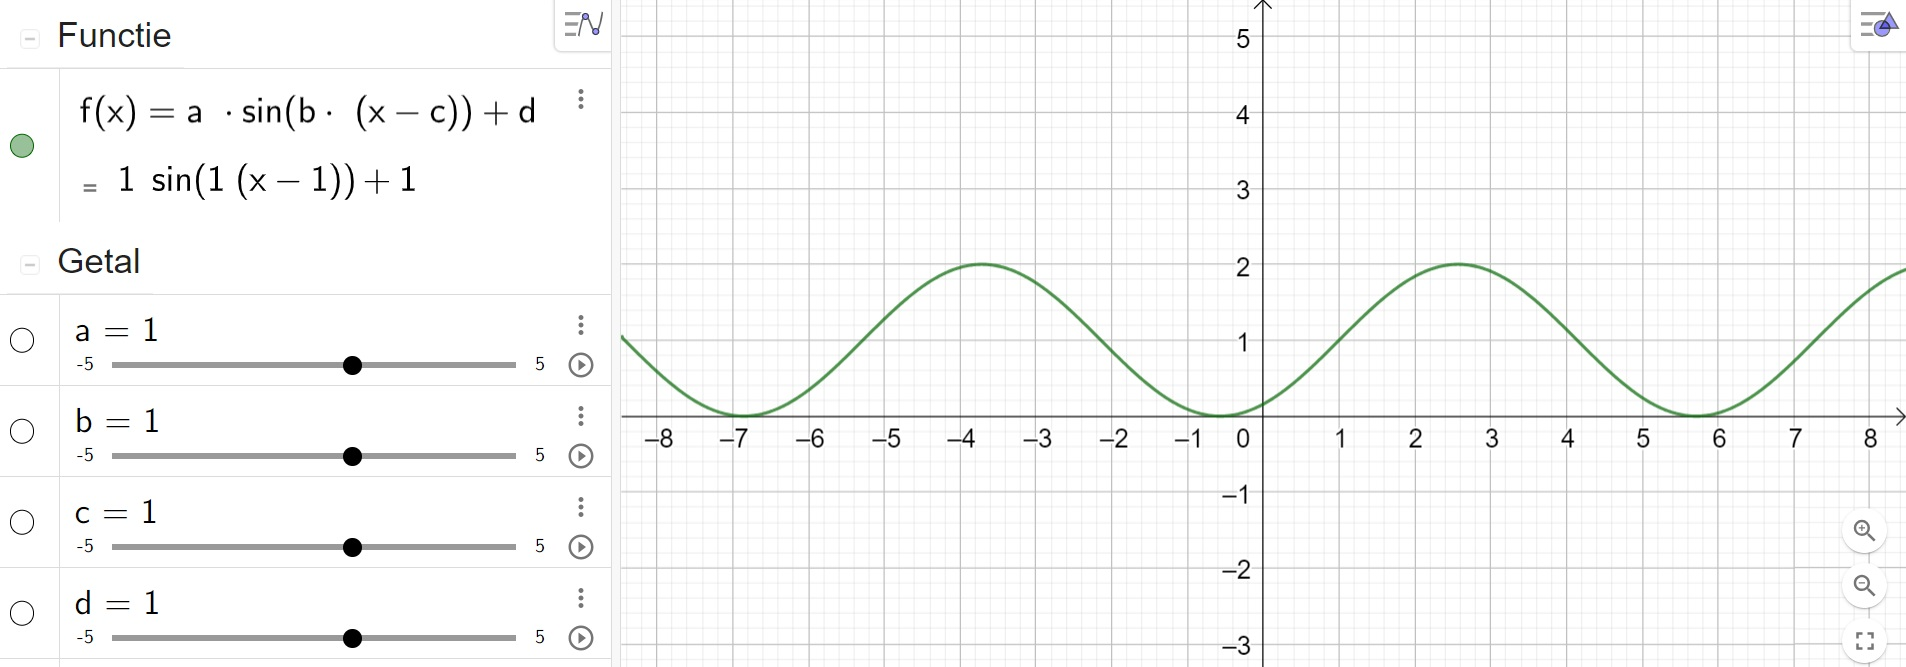
\includegraphics[width=0.9\textwidth]{img/Sinusfunctieabcd.jpg}
        \end{center}
        Het is bij het ingeven van dit voorschrift wel belangrijk dat de nodige maaltekens ingevoerd worden. Anders zal GeoGebra immers in de war zijn: GeoGebra interpreteert asin als boogsinus en $b(x-c)$ als de functie $b$ waarbij $x-c$ ingevuld wordt in het voorschrift.}
        \vraag{Experimenteer nu met elk van de schuifknoppen. Je kunt dit doen door het bolletje handmatig te verschuiven of door op \circled{$\blacktriangleright$} te klikken. Wat is het effect van elke parameter op de grafiek?}
        \antwoord{$a$ heeft een invloed op de hoogte van de golf of de amplitude. $b$ heeft een invloed op de lengte van de golf of de periode. $c$ en $d$ zorgen respectievelijk voor een horizontale en verticale verschuiving van de grafiek.}
        \vraag{Er zijn twee waardes van deze parameters waarbij je geen golvende grafiek ziet maar een rechte. Welke waardes zijn dit?}
        \antwoord{Dit gebeurt bij $a=0$ en ook bij $b=0$.}
        \vraag{De formules van tegengestelde, supplementaire en antisupplementaire hoeken laten ons toe om zulke voorschriften om te vormen naar (realistische) situaties waarbij $a$ en $b$ positief zijn. Laat nu de positieve waarde van de parameter $b$ veranderen. Kun je de getalwaarde van $b$ aflezen op de grafiek?}
        \antwoord{Je kunt de getalwaarde van $b$ niet rechtstreeks aflezen op de grafiek maar wel de golflengte. Als $b$ groter wordt, dan wordt de golflengte kleiner. De periode van de standaard sinusfunctie is $2 \pi$. De periode van de functie is $\dfrac{2\pi}{b}$. De getalwaarde van $b$ bepaalt de periode maar is er niet aan gelijk.\\
        Wanneer $b$ ook negatief (maar niet nul) kan zijn, dan is $\dfrac{2\pi}{|b|}$ de periode. Om eventuele verwarring met de negatieve $b$-waarden te vermijden, kan je eerst de minimale en maximale waarden van de schuifknop aanpassen via de knop $\ \vdots \ $ zoals hieronder.
        \begin{center}
        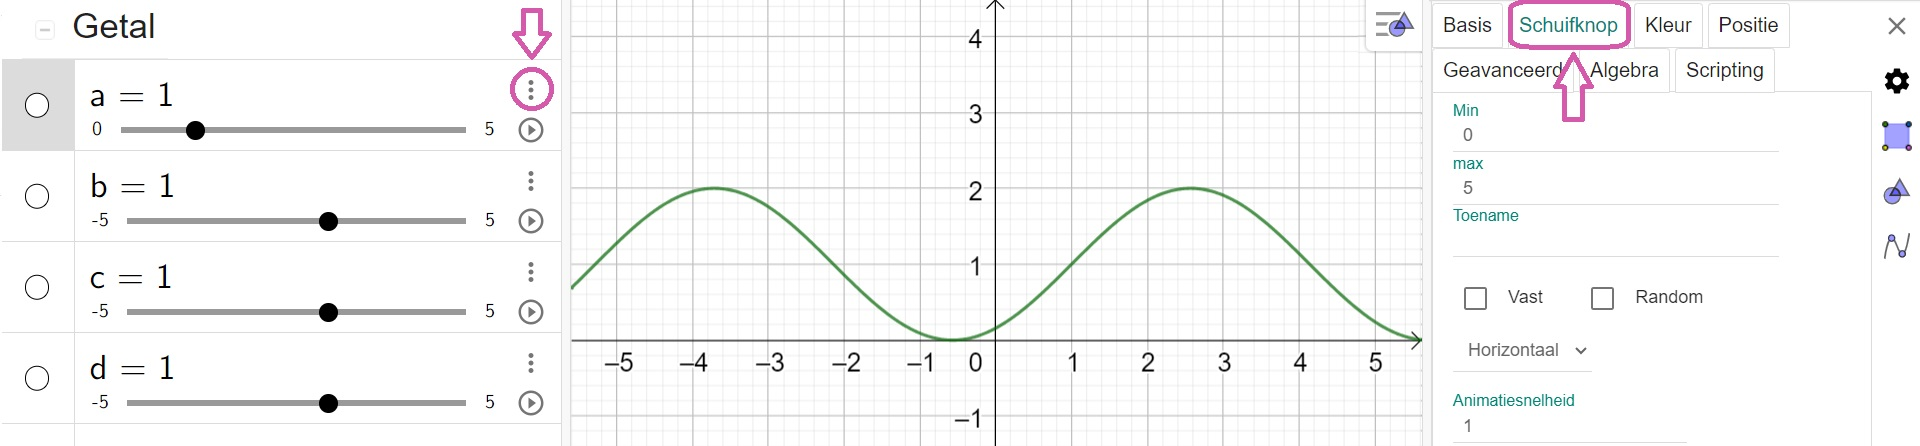
\includegraphics[width=0.9\textwidth]{img/Sinusfunctieschuifbalk.jpg}
        \end{center} }
        \vraag{In vraag 1 en 2 onderzochten we het effect van de parameters $a$, $b$, $c$ en $d$ op de grafiek. We merkten dat de grafiek van $y= f(bx)$ bekomen wordt uit $y=f(x)$ door een horizontale uitrekking ten opzichte van de $y$-as. Bij de functie $y=\sin \big( b \cdot (x-c) \big)$ lijk je uit te rekken ten opzichte van de rechte $x=c$. Wat vertelt je dit over de volgorde van de transformaties die we nodig hebben om $y=\sin(x)$ om te vormen naar $y=\sin \big( b \cdot (x-c) \big)$ ? Kies $a=1$ en $d=0$ als je dit visueel wilt onderzoeken.}
        \antwoord{We moeten eerst horizontaal uitrekken ten opzichte van de $y$-as en en daarna horizontaal verschuiven.}
        \vraag{Hoe zou het voorschrift eruit zien als we de grafiek van $y=\sin(x)$ eerst horizontaal verschuiven met $c$ eenheden naar rechts en daarna horizontaal uitrekken met factor $b$?}
        \antwoord{Dan heb je $y=\sin(bx-c)$. De haakjes zijn dus van belang!}
     \end{vraagenantwoord}
\end{lesactiviteit}

\begin{lesactiviteit}{Algemene sinusfunctie bij richtingen zonder component wiskunde}
\begin{vraagenantwoord}
    \vraag{Teken in GeoGebra de grafieken van de functies met voorschrift $f(x) = \sin(x)$ en $g(x)=a \cdot \sin(x)$. Wat doet GeoGebra met deze parameter $a$?}
        \antwoord{GeoGebra cre\"eert een schuifknop voor $a$. Deze loopt van $-5$ tot $5$ en toont nu de waarde 1.\\
        \begin{center}
        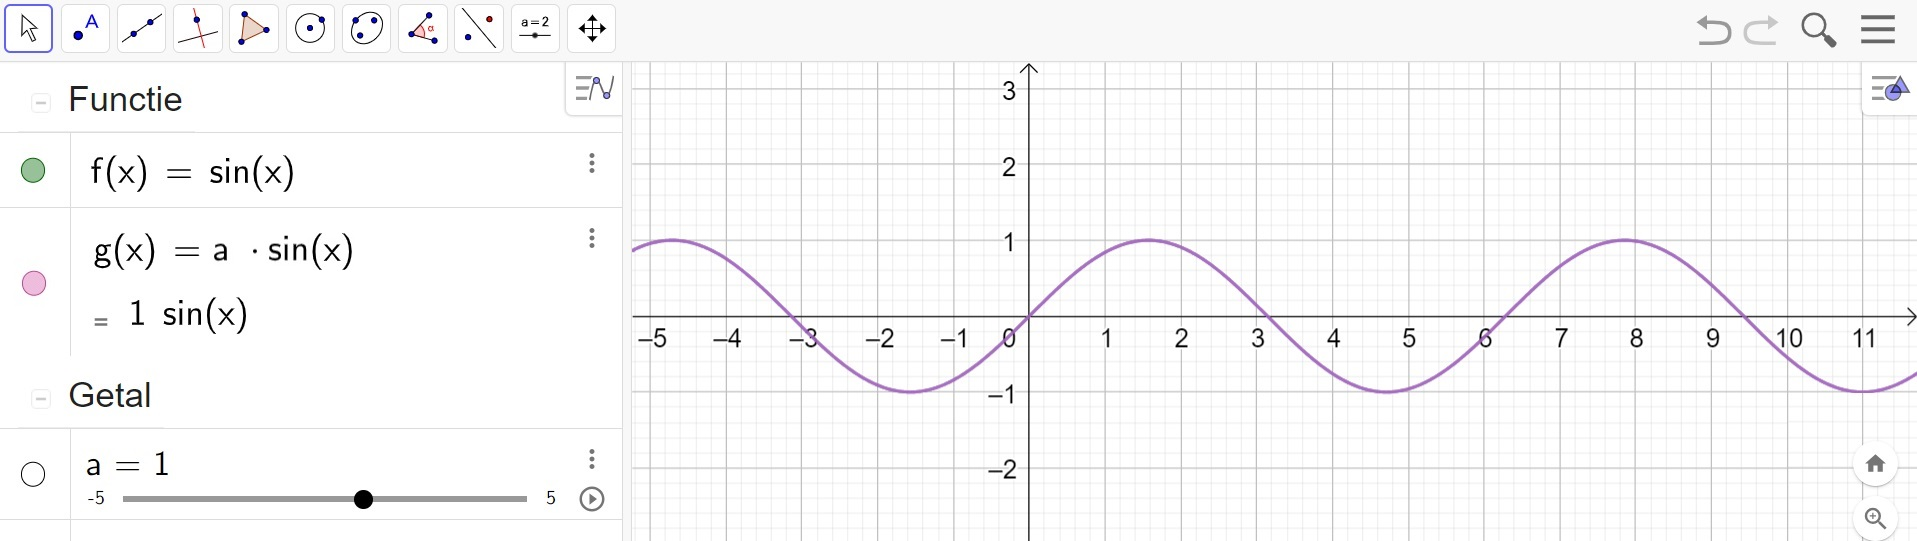
\includegraphics[width=0.9\textwidth]{img/Sinusfunctieenkela.jpg}
        \end{center}
        Het is bij het ingeven van dit voorschrift wel belangrijk dat de nodige maaltekens ingevoerd worden. Anders zal GeoGebra immers asin interpreteren als de functie met naam asin in de plaats van het product van het getal a met de functie sin.}
        \vraag{Hoe komt het dat we maar 1 grafiek zien?}
        \antwoord{Als $a=1$ dan is $g(x)=\sin(x)=f(x).$}
        \vraag{Verander nu de waarde van $a$. Je kunt dit doen door het bolletje handmatig te verschuiven of door op \circled{$\blacktriangleright$} te klikken. Wat is het effect hiervan op de grafiek?}
        \antwoord{We zien een verticale uitrekking met factor $|a|$, dat is de amplitude of de hoogte van de golf. Als $a$ negatief is, dan hebben we bovendien een spiegeling over de $x$-as. Je kan deze negatieve $a$-waarden uitsluiten in Geogebra door de minimale waarde van de schuifknop aan te passen naar 0 via de knop $\ \vdots \ $ zoals hieronder.
        \begin{center}
        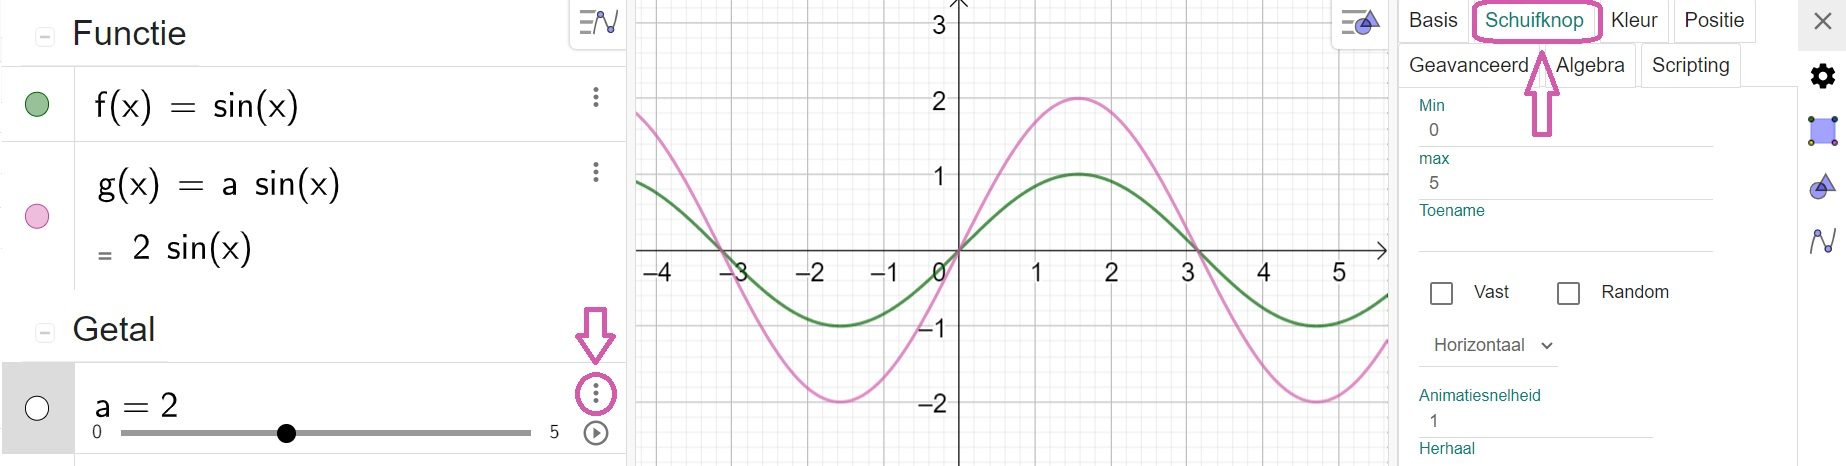
\includegraphics[width=0.9\textwidth]{img/Sinusfunctieschuifbalkenkela.jpg}
        \end{center}}

        \vraag{Teken nu de grafiek van $h(x)=a \cdot sin(b \cdot x)$. Er verschijnt een schuifknop voor de onbekende $b$. Welke transformatie van de grafiek bekom je als je de waarde van $b$ verandert?}
        \antwoord{We zien een horizontale uitrekking of samendrukking. Als de waarde van $b$ kleiner wordt, dan wordt de golf langer, als de waarde van $b$ groter wordt, dan wordt de golf korter.}
        \vraag{Teken nu de grafieken van $i(x)=a \cdot \sin \big(b (x-c) \big)$ en $j(x)=a \cdot \sin \big(b (x-c) \big) +d$. Welke transformaties komen overeen met de letters $c$ en $d$?}
        \antwoord{$c$ zorgt voor een horizontale verschuiving, $d$ zorgt voor een verticale verschuiving.}
\end{vraagenantwoord}
\end{lesactiviteit}
\begin{multicols}{2}
\subsection{Afgeleiden en integralen}

\end{multicols}
\begin{lesactiviteit}{Afgeleiden en integralen bij een gedempte oscillator}
    Een massa hangt in rust aan een veer. Je trekt de massa eerst naar beneden en laat ze dan los. De massa oscilleert nu omhoog en omlaag. Door wrijving dooft deze oscillatie geleidelijk uit. De snelheid $v$ (in m/s) wordt in functie van de tijd $t$ (sinds het loslaten en gemeten in s) gegeven door
    \[ v(t) = e^{\frac{-t}{10}} \cdot \sin(3t) \]
    \begin{vraagenantwoord}
        \vraag{Wat is de hoogste snelheid die de massa bereikt? Onderzoek dit met GeoGebra.}
        \antwoord{We weten dat dit extremum bereikt wordt binnen de eerste 2 seconden. Dat zien we aan de grafiek en omdat $\sin(t)$ een eerste periode doorloopt in $\left[0,\dfrac{2\pi}{3}\right[$. Via het commando \emph{Extrema(v,0,2)} vinden we een maximale snelheid van 0,9495m/s. Je kunt extrema ook vinden via het menu linksboven (zie afbeelding hieronder).}
        \vraag{Hoe kun je de co\"ordinaten van de extrema tonen op de grafiek?}
        \antwoord{Je selecteert het punt en kiest bij instellingen voor Naam \& waarde als label.\\
        \begin{center}
        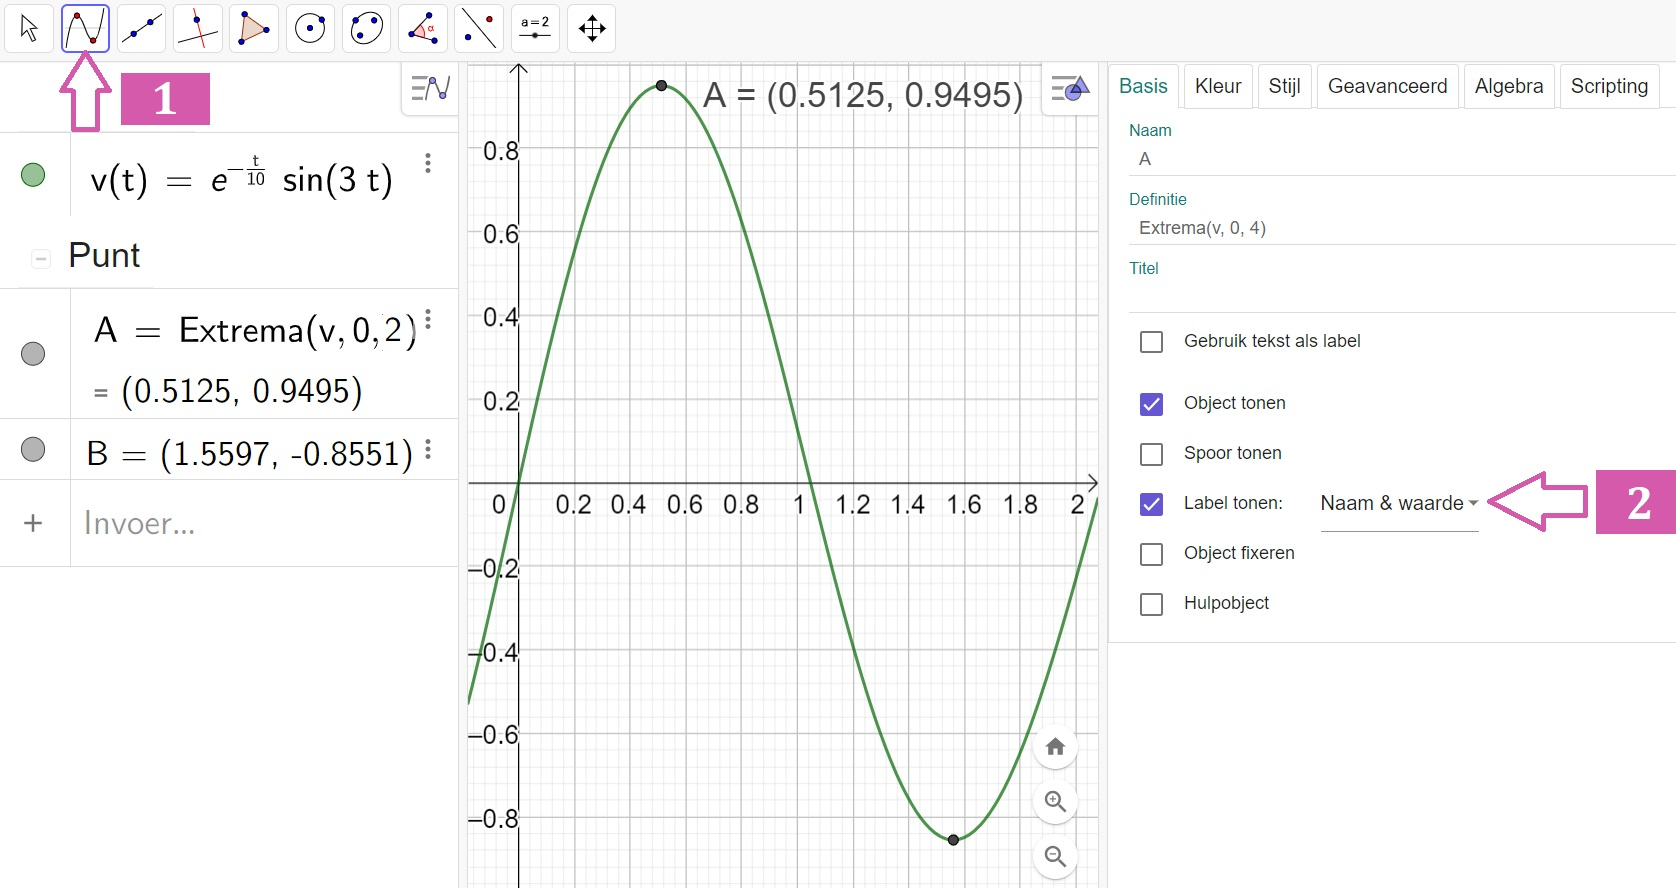
\includegraphics[width=0.9\textwidth]{img/Extremazoeken.jpg}
        \end{center}
        }
        \begin{multicols}{2}
        \vraag{Wat weet je over $v'(t)$ bij dit extremum?}
        \antwoord{Aangezien $v$ overal afleidbaar is, geldt $v'(t)=0$ bij elk extremum. We kunnen dit nagaan via GeoGebra. Daar vinden we de afgeleide functie van $v$ door $v'$ te typen en vinden we de $x$-co\"ordinaat van het punt $A$ via $x(A)$.
        \columnbreak
        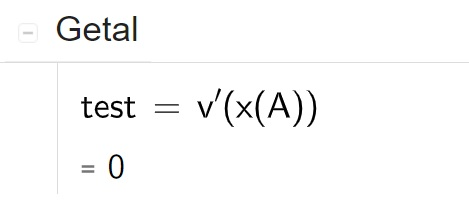
\includegraphics[width=0.45\textwidth]{img/Testafgeleidenul.jpg}
        }
        \end{multicols}
        \vraag{We hebben $v(t)=0$ voor $t=\dfrac{k \pi}{3}$ voor alle $k \in \mathbb{N}$. Wat is de praktische interpretatie hiervan?}
        \antwoord{De massa wisselt dan van bewegingszin bij alternerend relatief maximale en relatief minimale hoogtes. De snelheidsfunctie is immers de afgeleide van de hoogtefunctie in dit voorbeeld.}
        \vraag{Na $\dfrac{2 \pi}{3}$ seconden bereikt de massa een relatief minimale hoogte. Dit is echter minder diep dan het punt waarop je de massa initieel hebt losgelaten. Hoe bereken je dit hoogteverschil?}
        \antwoord{De snelheidsfunctie is de afgeleide van de hoogtefunctie. Om het verschil in hoogte te berekenen gebruiken we dus een integraal. Concreet zoeken we de volgende integraal via GeoGebra
        \[ \int_0^{\frac{2\pi}{3}} v(t) dt\]
        \begin{center}
        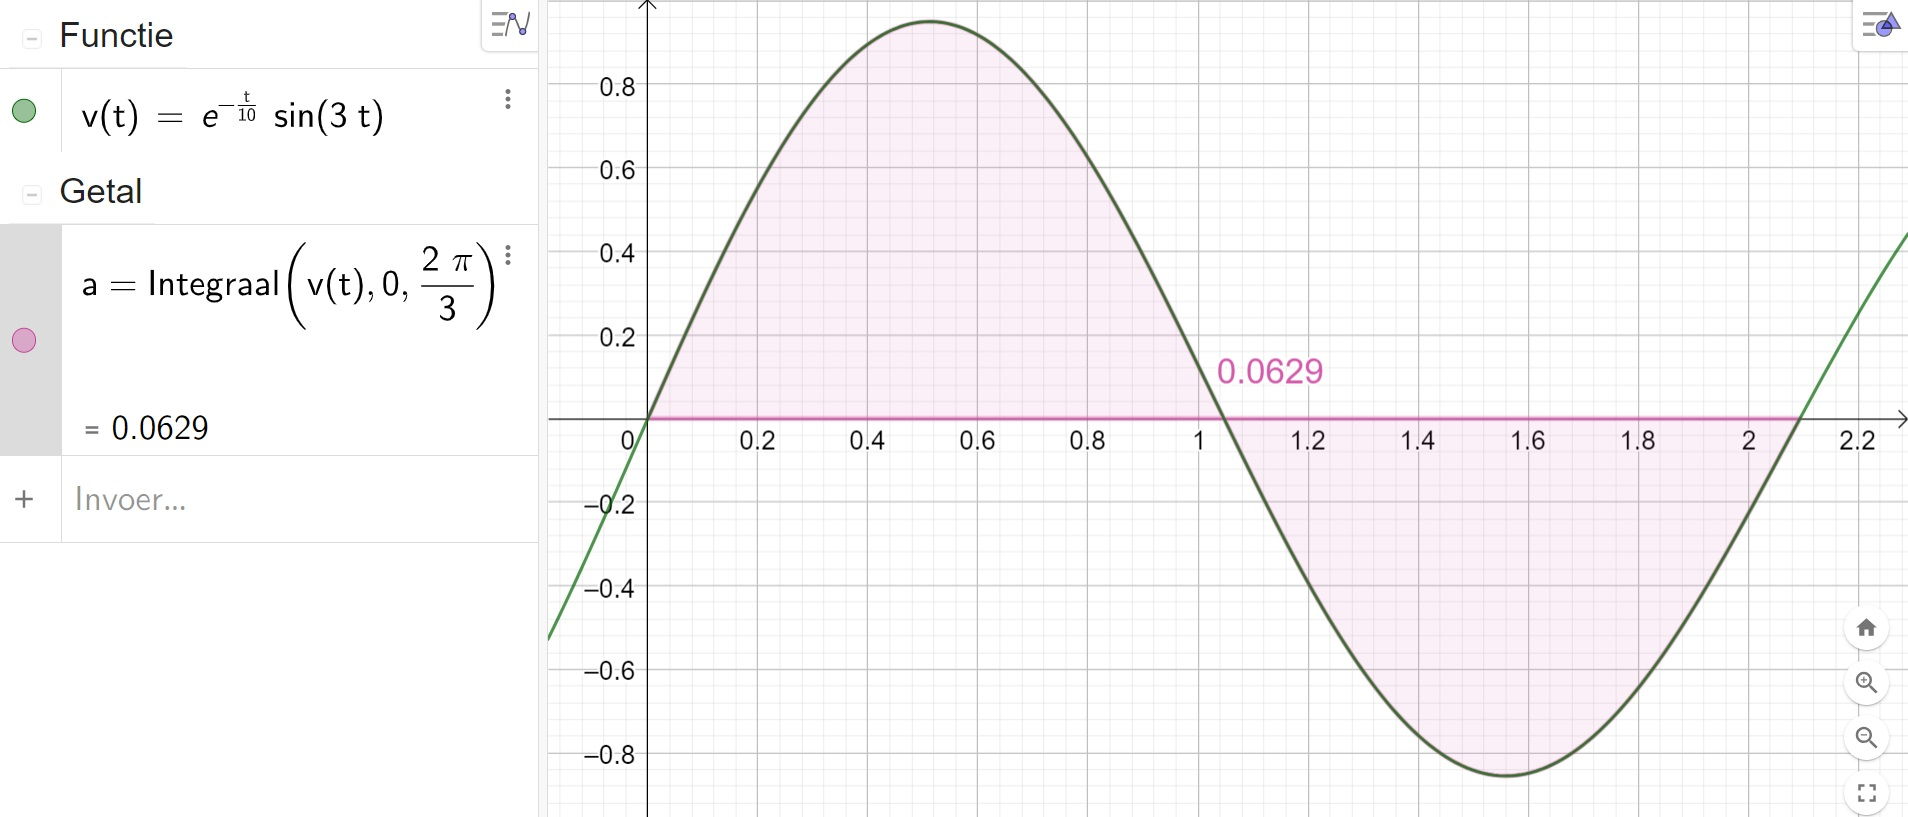
\includegraphics[width=0.9\textwidth]{img/Integraaleindig.jpg}
        \end{center}
        Er is dus een hoogteverschil van 6,29 cm.}
        \vraag{Kun je op een analoge manier berekenen hoe ver je de massa initieel naar beneden hebt getrokken?}
        \antwoord{Als we de tijd oneindig lang laten doorlopen, dan zal de massa (in de limiet) tot stilstand komen in de rustpositie. De originele uitrekking vinden we dus via de volgende integraal:
        \[ \int_0^{+ \infty} v(t) dt \]
        Op GeoGebra geven we dit in via Integraal(v(t),0,$\infty$). Het $\infty$-symbool vind je bijvoorbeeld via het digitale toetsenbord of door \emph{inf} te typen bij de invoer. Het algebravenster heeft echter problemen met het uitrekenen van deze oneigenlijke integralen. Daarom schakelen we over naar het CAS-venster waar GeoGebra de berekening wel kan doen.
        \begin{center}
        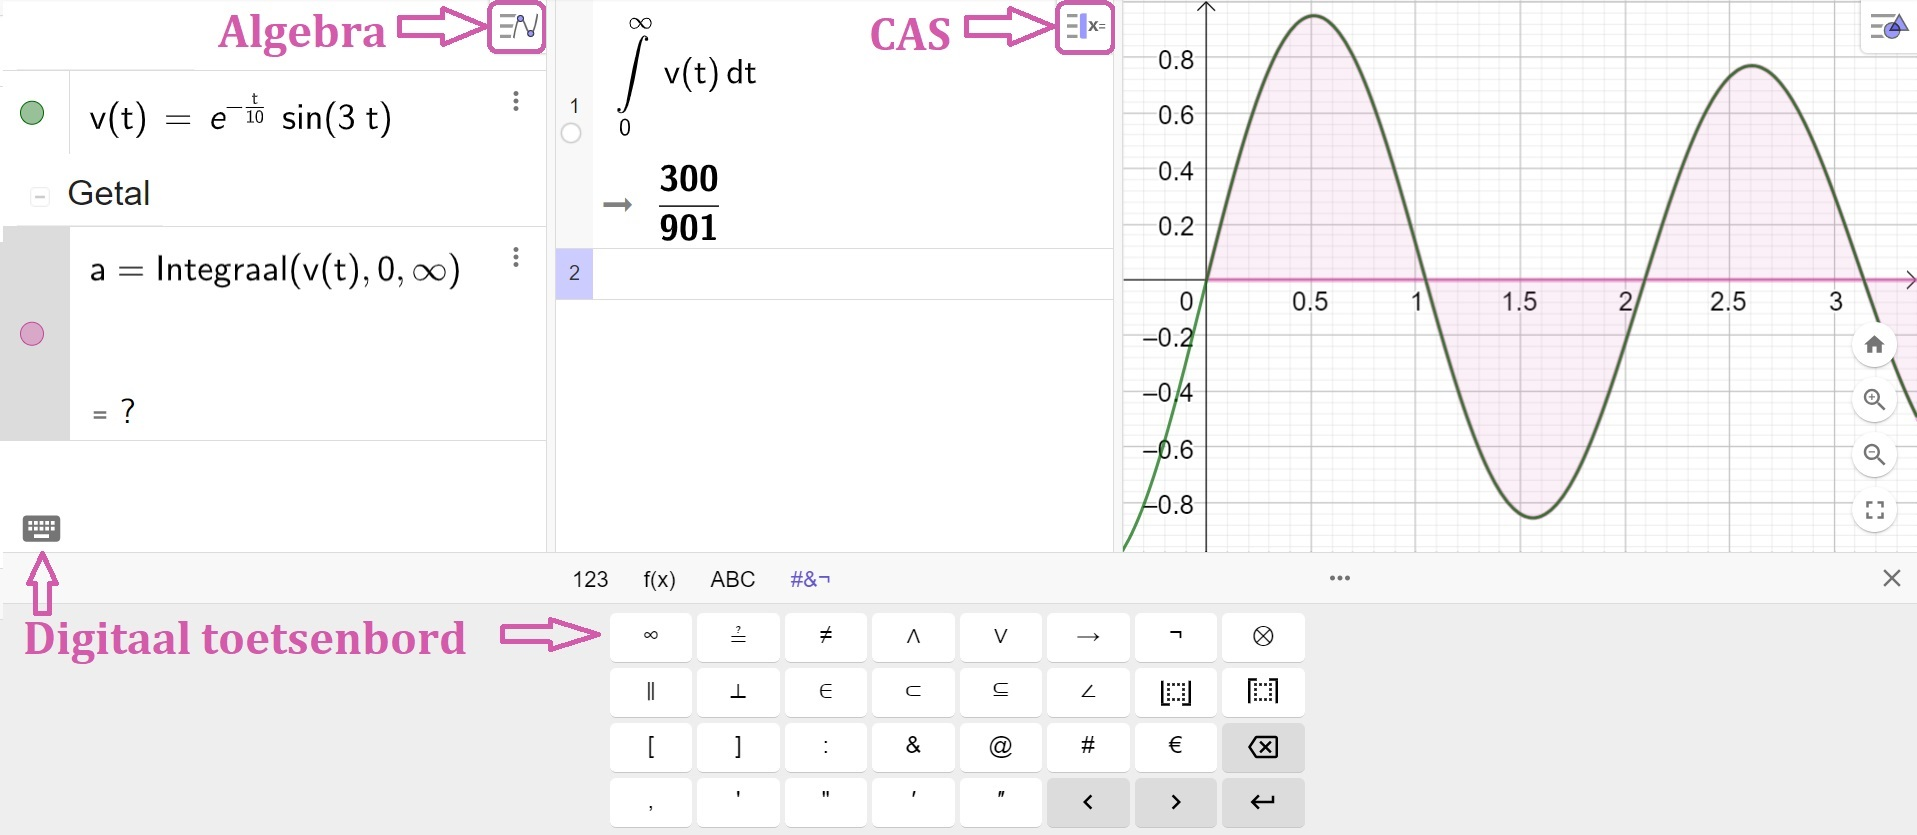
\includegraphics[width=0.9\textwidth]{img/Integraaloneindig.jpg}
        \end{center}
        We concluderen dat we de veer over ongeveer $\dfrac{300}{901}$cm of ongeveer 33,3 cm hadden uitgerekt. Wanneer het volstaat om enkel een benaderende waarde te kennen, dan kan je ook een groot getal (zoals 999) invoeren als bovengrens van de integraal. Dat kan wel in het algebravenster.}
    \end{vraagenantwoord}
\end{lesactiviteit}

\begin{multicols}{2}

Aanvullend op bovenstaande lesactiviteit vermelden we dat CAS nog tal van andere extra functionaliteiten heeft die niet mogelijk zijn in het algebravenster. 
\begin{itemize}
    \item Onbepaalde integralen uitrekenen via Integraal(functievoorschrift) 
    \item Splitsen in partieelbreuken via Partieelbreuken(rationale functie)
\end{itemize}


\subsection{Matrices}
Matrices worden in de derde graad ge\"introduceerd als een tabel met getallen waarmee gerekend kan worden. Na het goed defini\"eren van de bewerkingen, wordt de meerwaarde duidelijk bij het beschrijven van evoluties van populaties en migratiepatronen. Een specifiek minimumdoel in alle richtingen waar matrices op het programma staat luidt dan ook `de leerlingen gebruiken matrixmodellen om evoluties te beschrijven'. Het gebruik van ICT is hier onontbeerlijk om de matrixproducten uit te rekenen zodat de focus kan liggen op het interpreteren. In voorbije edities van Uitwiskeling (27/3, 19/1, 13/3 en 05/1) werden reeds enkele voorbeelden uitgewerkt met een grafisch rekentoestel. In de lesactiviteit hieronder illustreren we hoe het met GeoGebra kan.  

 \end{multicols}

\begin{lesactiviteit}{Populatiegroei onderzoeken met matrices in GeoGebra}
    Een kolonie van een diersoort kun je volgens leeftijd indelen in drie groepen: jong (tot 1 jaar oud), volwassen (tussen 1 en 2 jaar oud) en senior (ouder dan 2 jaar). Het aandachtig bestuderen van deze kolonie heeft geleid tot de volgende vaststellingen.
    \begin{itemize}
        \item De jonge diertjes brengen tegen de eerste winter elk gemiddeld twee nakomelingen voort. De helft van de jonge diertjes overleeft hun eerste winter echter niet.
        \item De volwassenen brengen tegen de volgende winter elk gemiddeld anderhalve nakomeling voort. Ook de helft van de volwassenen haalt het einde van de winter niet.
        \item De oudste dieren zijn in hun laatste levensjaar actief bezig met voortplanting en brengen elk gemiddeld vijf nakomelingen voort. Geen enkele senior overleeft een derde winter. 
    \end{itemize}

    \begin{vraagenantwoord}
        \vraag{Geef de overgangsmatrix $L$ die de evolutie van de populatie dieren winter na winter bepaalt.}
        \antwoord{In de eerste rij worden de \emph{vruchtbaarheidscijfers} geplaatst (nieuwe jongeren door elke leeftijdsgroep), onder de diagonaal staan de \emph{overlevingskansen} (overgang naar de volgende leeftijdsgroep). Het diagonaalelement rechtsonder is gelijk aan 0 want de oudste groep heeft geen overlevingskans. weer. 
        $$  \begin{array}{ccc} & & \textcolor{gray}{naar} \\
        L = & \begin{pmatrix}
        2 & 1{,}5 & 5 \\
        0{,}5 & 0 & 0 \\
        0 & 0{,}5 & 0
        \end{pmatrix}  &  \begin{array}{c} \textcolor{gray}{J} \\ \textcolor{gray}{V} \\ \textcolor{gray}{S} \end{array} \\
        \textcolor{gray}{van} & \begin{array}{ccc} \;\textcolor{gray}{J}\;\; & \;\textcolor{gray}{V}\; & \;\;\textcolor{gray}{S}\; \end{array} & \\ \end{array}$$}

        \vraag{Onderzoekers stellen een groep van 10 jongeren, 10 volwassenen en 10 senioren samen. Hoeveel dieren van elke leeftijdsgroep verwacht je na de volgende winter te hebben?}
  \antwoord{Noteer de beginpopulatie als de kolomvector $X_0 = \begin{pmatrix}
        10\\
        10 \\
        10
        \end{pmatrix} \begin{array}{c} \textcolor{gray}{J} \\ \textcolor{gray}{V} \\ \textcolor{gray}{S} \end{array}$. \\
        De populatie na \'e\'en jaar noteren we als $X_1$ en kan berekend worden via het matrixproduct $X_1 = L \cdot X_0$. Wanneer leerlingen nog niet vertrouwd zijn met populatiematrices, loont het de moeite om eerst deze vraag zonder het defini\"eren van een populatiematrix uit te rekenen om in die berekening inderdaad een matrixproduct te herkennen.\\[6pt]
        %
        Om GeoGebra hier in te schakelen, doe je het volgende. In het rekenblad van GeoGebra Classic kun je de elementen van een matrix ingeven in cellen, deze cellen selecteren en als matrix defini\"eren via de knop \emph{Maak een matrix}. Als je kiest voor \emph{Afhankelijke objecten} worden niet de waarden maar de cellen zelf gekoppeld aan de elementen van de matrix. Je kunt zo de elementen van de matrix aanpassen door in het rekenblad de waarde van een cel te veranderen. Vervolgens kun je met gedefinieerde matrices berekeningen uitvoeren in het algebravenster. Zo krijg je na de eerste winter 85 jongeren, 5 volwassenen en 5 senioren.}

            $$\vcenter{\hbox{\includegraphics[width=0.35\textwidth]{img/matrices/matrix12.png}}} \qquad \vcenter{\hbox{\includegraphics[width=0.4\textwidth]{img/matrices/matrix3.png}}}$$
            %
            $$\vcenter{\hbox{\includegraphics[width=0.42\textwidth]{img/matrices/matrix4.png}}} \qquad
            \vcenter{\hbox{\includegraphics[width=0.22\textwidth]{img/matrices/matrix5.png}}} \qquad\qquad
            \vcenter{\hbox{\includegraphics[width=0.11\textwidth]{img/matrices/matrix6.png}}}$$
        
        \vraag{Hoeveel dieren zullen er naar verwachting zijn na drie winters?}
        \antwoord{Bereken via GeoGebra $X_3 = L^3 \cdot X_0$ (of via $X_2 = L\cdot X_1$ en vervolgens $X_3 = L \cdot X_2$). \\
        %
        $$\vcenter{\hbox{\includegraphics[width=.15\textwidth]{img/matrices/matrix7.png}}} \qquad\qquad \vcenter{\hbox{\includegraphics[width=.175\textwidth]{img/matrices/matrix8.png}}}$$
        %
        % $$X_3 = \begin{pmatrix}
        % 481{,}25\\
        % 101{,}25 \\
        % 21{,}25
        % \end{pmatrix} \begin{array}{c} \textcolor{gray}{J} \\ \textcolor{gray}{V} \\ \textcolor{gray}{S} \end{array} $$
        Merk op dat hier `kwartjes van dieren' in voorkomen. Dit komt omdat populatiematrices een model zijn en dus \emph{voorspellend} werken, niet als een \emph{exacte beschrijving}. De bekomen getallen moeten daarom steeds als een verwachte waarde ge\"interpreteerd worden. In totaal verwacht men dus dat de kolonie zal bestaan uit $603{,}75 \approx 604$ dieren na drie winters. Dit kan via het commando \emph{Som($X_3$)} door GeoGebra berekend worden.} 

        \vraag{Onderzoek en bespreek de populatiegroei op lange termijn.}
        \antwoord{Door de populatie $X_n$ na $n$ winters voor verschillende waarden van $n \in \mathbb{N}_0$ uit te rekenen, is snel duidelijk dat er geen stabiel evenwicht optreedt. De populatie groeit onbegrensd, althans volgens dit wiskundig model waarbij biologische en ecologische factoren zoals de voedselvoorraad niet in rekening gebracht zijn. \\[6pt]
        %
        Echter, door de populatie in twee opeenvolgende jaren te beschouwen, bijvoorbeeld na 8 en 9 winters zoals voorgesteld door de matrices $X_8$ en $X_9$, kun je zien dat de leeftijdsgroepen aangroeien met een factor die ongeveer gelijk is. Deze factor kun je bepalen door via GeoGebra de overeenkomstige matrixelementen te delen zoals ge\"illustreerd hieronder. Hierbij staat $X_9(i,j)$ voor het element in de $i$-de rij en $j$-de kolom van $X_9$. Er geldt $X_{n+1} \approx 2{,}5\cdot X_n$ voor $n \gg 1$. Hoe verder je doorgaat in de tijd, hoe beter de aangroeifactor 2{,}5 benadert. Deze factor wordt een \emph{eigenwaarde} van de overgangsmatrix genoemd. \\[6pt]
        %
        Noot: in GeoGebra kun je matrices `delen', al wordt dit element per element uitgevoerd. Enige waakzaamheid is geboden bij het gebruik hiervan aangezien deze operatie niet de tegenhanger is van de aangeleerde matrixvermenigvuldiging.  
        %
        $$\vcenter{\hbox{\includegraphics[width=.225\textwidth]{img/matrices/X8.png}}} \qquad\qquad \vcenter{\hbox{\includegraphics[width=.225\textwidth]{img/matrices/X9.png}}}$$
        %
         $$\vcenter{\hbox{\includegraphics[width=.18\textwidth]{img/matrices/verhouding.png}}} \qquad\qquad \vcenter{\hbox{\includegraphics[width=.16\textwidth]{img/matrices/verhouding1.png}}}\qquad \vcenter{\hbox{\includegraphics[width=.16\textwidth]{img/matrices/verhouding2.png}}}\qquad \vcenter{\hbox{\includegraphics[width=.157\textwidth]{img/matrices/verhouding3.png}}}$$
        }
         \vraag{De verhoudingen van de leeftijdsgroepen onderling evolueren naar een constante. Bepaal deze constante verhouding.}
         \antwoord{Analoog aan de vorige vraag. Door het berekenen van de populatie na een groot aantal winters en de elementen onderling door elkaar te delen, kun je de evolutie naar onderlinge verhoudingen van $25:5:1$ vinden. Er zijn dus 25 keer zoveel jongeren en 5 keer zoveel volwassen als senioren na verloop van tijd. Deze verhouding kan als kolomvector $X_\infty$ genoteerd worden. Dit wordt een \textit{eigenvector} van de populatiematrix bij eigenwaarde 2{,}5 genoemd wegens $L\cdot X_\infty = 2{,}5 \cdot X_\infty$.    
         $$\vcenter{\hbox{\includegraphics[width=.15\textwidth]{img/matrices/verhouding4.png}}}\qquad \vcenter{\hbox{\includegraphics[width=.15\textwidth]{img/matrices/verhouding5.png}}} \qquad\qquad X_\infty = \begin{pmatrix}
        25 \\
        5 \\
        1 
        \end{pmatrix} \begin{array}{c} \textcolor{gray}{J} \\ \textcolor{gray}{V} \\ \textcolor{gray}{S} \end{array}$$
         . 
         }
    \end{vraagenantwoord}
\end{lesactiviteit}
\begin{multicols}{2}



 \section{Appendix: technisch gesproken}

\subsection*{Examenmodus} 
Bij toetsen laat je de leerlingen best GeoGebra in de examenmodus zetten op hun apparaat. Ze kunnen dan alle functionaliteiten van GeoGebra gebruiken zonder dat ze daarbij toegang hebben tot het internet of andere software. Cambré en GeoGebra Team German (z.d.) schreven een heel handig online GeoGebraboek over de examenmodus, met titel `GeoGebra voor toetsen'. In dat boek leggen ze overzichtelijk uit wat de examenmodus precies is en hoe je die activeert. Ze geven er ook praktische tips voor het gebruik in de klas. Je vindt het boek op de website \url{geogebra.org}.

\subsection*{Online account}
Je kunt met GeoGebra werken in verschillende versies, zowel online als offline en op elk mogelijk toestel (pc, tablet, smartphone). Vanuit alle versies kun je documenten zowel online opslaan als op je computer. Op \url{geogebra.org} kun je een online gebruikersaccount aanmaken. Dit laat je toe om GeoGebra-bestanden in de cloud op te slaan, wat erg handig is om lesmateriaal te delen met leerlingen of collega's. Een account aanmaken, doe je door rechts bovenaan op \emph{Aanmelden} te klikken. Het kan ook via \emph{Profiel} in de linkerkolom. Eens je een account hebt, kun je via \emph{$+$Creëer} of \emph{online opslaan} een nieuw werkblad maken op het materialenplatform van GeoGebra. Hoe je dit doet, lees je in één van de initiatiehandleidingen die je vindt op de openingspagina van \url{geogebra.org}.

\subsection*{Initiatiehandleidingen}
Met GeoGebra leren werken als leraar wordt meer en meer een tweesporenopdracht.
Oorspronkelijk was GeoGebra voor leraren vooral een tool om afbeeldingen te maken voor cursussen, toetsen, examens en om toonbestanden te maken voor de lessen.
Meer en meer profileert GeoGebra zich daarnaast echter ook als een grafische rekenmachine voor dagelijks gebruik door leerlingen in de klas (vaak op de smartphone of laptop). Mee daardoor heb je verschillende versies van GeoGebra, zoals bijvoorbeeld Rekenmachine Suite en GeoGebra Klassiek, die elk hun eigen functionaliteiten hebben.

Om je wegwijs te maken, vind je op de openingspagina van \url{geogebra.org} verschillende handige initiatiehandleidingen. Een heel goed startpunt is het GeoGebraboek `GeoGebra gebruiken' (Cambré, z.d.).


\subsection*{Aanbevolen materiaal en App downloads}
Nog op de openingspagina van \url{geogebra.org} vind je \emph{Aanbevolen materiaal}. Hier zie je de ongelooflijk uitgebreide collectie lesmaterialen van Cambré (z.d.), per graad gerangschikt. Voor elk onderwerp vind je er lesmaterialen die je online kunt gebruiken of kunt downloaden voor offline gebruik. Je kunt ook de zoekfunctie bovenaan de webpagina gebruiken om materialen te zoeken.

Verder vind je op de openingspagina nog een link naar \emph{App Downloads}. Deze link brengt je naar een pagina met alle GeoGebra-apps. Je kunt daar kiezen om een app te downloaden naar je apparaat of om deze app online te starten.




\subsection*{Soms loopt het mis}
Tot slot geven we ook even mee dat het gebruikte toestel soms een invloed heeft op de werking van GeoGebra. Wanneer je bijvoorbeeld werkt met een tablet zonder fysiek toetsenbord, dan ben je volledig afhankelijk van het digitale toetsenbord dat door GeoGebra voorzien wordt (zie bijvoorbeeld de lesactiviteit van de gedempte oscillator). Het risico bestaat hierbij dat het knopje van het digitale toetsenbord plots verdwenen is en je niets meer kunt invoeren. De ervaring leert dat dit risico re\"eel is, maar het komt heel zelden voor. In dit geval is het herstarten van de app vaak de snelste oplossing. Wanneer je bovendien werkt met toestellen met een klein werkgeheugen, dan kan GeoGebra moeite hebben met werken in 3D of bestanden waarin een parameter gebruikt wordt. Hier ligt de oplossing vaak in het gebruik van \url{geogebra.org/classic}.

 


 \end{multicols}

 \begin{bronnen}

\item Cambré, C. (z.d.). \emph{GeoGebra CAS}. GeoGebra. Geraadpleegd op 3 september 2023, van \url{https://www.geogebra.org/m/syfg22j8}

\item Cambré, C. (z.d.). \emph{GeoGebra gebruiken}. GeoGebra. Geraadpleegd op 3 september 2023, van \url{https://www.geogebra.org/m/ermrfpec}


\item Cambré, C., GeoGebra Team German.  (z.d.) \emph{GeoGebra voor toetsen}. Geogebra. Geraadpleegd op 3 september 2023, van \url{https://www.geogebra.org/m/scntsjc9}

\item Coussement, E. (2023). Correlatie en regressie met GeoGebra Suite. \emph{Wiskunde en Onderwijs 49/194}, 7-12.

\item Forman, S. (2000). \emph{Sports Reference. Sports Stats, fast, easy, and up-to-date}. Sports Reference.\\ \url{https://www.sports-reference.com/}

 \item Gheysens, L. (2012, 11 juni). \emph{ICT-leerlijn (met GeoGebra)}. Gnomon. \url{http://blogimages.bloggen.be/gnomon/attach/153368.pdf}

\item Gunawan, F. (2012). Two-Vehicle Dynamics of the Car-Following Models on Realistic Driving Condition. \emph{Journal of Transportation Systems Engineering and Information Technology. 12.} 77-83.


 %\item 2000 reeds gemaakte GeoGebrafiguren per graad (kan inspireren) ((Ik ben vergeten waar ik dit ben tegengekomen.)) Dat is bij de online GeoGebraboeken van Chris Cambré.

\item Kesselaers, G., Van Leemput, G., \& Roels, J. (1999). De stelling van Pythagoras en een geïntegreerde aanpak in het derde jaar. \emph{Uitwiskeling 15-2}, 12-37.



 \end{bronnen}



